\documentclass [preprint]{sigplanconf}
\usepackage[latin1]{inputenc}
\usepackage{amsmath}
\usepackage{xspace}
\usepackage{amsfonts}
\usepackage{amssymb}
\usepackage{latexsym}
\usepackage{graphicx}
\usepackage[latin1]{inputenc}
\usepackage{amsmath,amsfonts,amssymb}
\usepackage{algorithm}
\usepackage[noend]{algpseudocode}
\usepackage{algorithm}
\usepackage{url}
\usepackage{amsmath, amsthm, amssymb}
\usepackage{color}
\usepackage{fancyvrb}
\usepackage{mathpartir}

\usepackage{caption}
\usepackage{subcaption}

\usepackage{tikz}
\usetikzlibrary{arrows,automata}
\usetikzlibrary{shapes.symbols}
\usetikzlibrary{shapes}

\newtheorem{theorem}{Theorem}

\theoremstyle{remark}
\newtheorem{example}{Example}

\theoremstyle{definition}
\newtheorem{definition}{Definition}

\newcommand{\civl}{{\sc civl}\xspace}
\newcommand{\boogie}{{\sc boogie}\xspace}
\newcommand{\zthree}{{\sc Z3}\xspace}
\newcommand{\casm}{{\sc casm}\xspace}
\newcommand{\why}{{\sc why}\xspace}

\makeatletter
\let\@copyrightspace\relax
\makeatother

\begin{document}

\special{papersize=8.5in,11in}
\setlength{\pdfpageheight}{\paperheight}
\setlength{\pdfpagewidth}{\paperwidth}

\conferenceinfo{CONF 'yy}{Month d--d, 20yy, City, ST, Country} 
\copyrightyear{20yy} 
\copyrightdata{978-1-nnnn-nnnn-n/yy/mm} 
\doi{nnnnnnn.nnnnnnn}

\title{Automated and modular refinement reasoning for concurrent programs}
\authorinfo{}{}{}

\maketitle


\newcommand{\Type}{\mathit{Type}}
\newcommand{\VarName}{\mathit{AllVar}}
\newcommand{\Var}{\mathit{Var}}
\newcommand{\Value}{\mathit{Value}}
\newcommand{\Expr}{\mathit{Expr}}
\newcommand{\StateExpr}{\mathit{Expr}}
\newcommand{\TransExpr}{\mathit{TransExpr}}
\newcommand{\LocalStateExpr}{\mathit{LocalExpr}}
\newcommand{\Spec}{\mathit{Spec}}
\newcommand{\Program}{\mathit{Program}}
\newcommand{\Prog}{\mathit{Prog}}
\newcommand{\ProcName}{\mathit{Proc}}
\newcommand{\ActionName}{\mathit{Action}}
\newcommand{\Proc}{\mathit{Proc}}
\newcommand{\proc}{\mathit{Pr}}
\newcommand{\Thread}{\mathit{Thread}}
\newcommand{\Body}{\mathit{Body}}
\newcommand{\Stmt}{\mathit{Stmt}}
\newcommand{\stmt}{\mathit{s}}
\newcommand{\locExpr}{\mathit{le}}
\newcommand{\exC}[1]{{\tt {#1}}}
\newcommand{\Frame}{F}
\newcommand{\Frames}{\overrightarrow{\Frame}}
\newcommand{\FrameCtxt}{\mathit{FC}}
\newcommand{\MakeFrames}[1]{\overrightarrow{#1}}

\newcommand{\ite}[3]{\mathit{if}\hspace{0.5mm}{#1}\hspace{0.5mm}\mathit{then}\hspace{0.5mm}{#2}\hspace{0.5mm}\mathit{else}\hspace{0.5mm}{#3}}
\newcommand{\while}[3]{\mathit{while}\hspace{0.5mm}\{#1\}\hspace{0.5mm}{#2}\hspace{0.5mm}\mathit{do}\hspace{0.5mm}{#3}}
\newcommand{\yield}[1]{\mathit{yield}\ #1}
\newcommand{\join}[1]{\mathit{join}\ #1}
\newcommand{\async}[1]{\mathit{async}\ #1}
\newcommand{\call}[1]{\mathit{call}\ #1}
\newcommand{\ablock}[2]{\mathit{ablock}\ {\{#1\}}\ {#2}\ }
\newcommand{\parcall}[2]{\mathit{call}\ {#1} || {#2}\ }
\newcommand{\assert}[1]{\mathit{assert}\ #1}
\newcommand{\assume}[1]{\mathit{assume}\ #1}
\newcommand{\havoc}[1]{\mathit{havoc}\ #1}
\newcommand{\goto}[1]{\mathit{goto}\ #1}
\newcommand{\fork}[1]{\mathit{par}\ #1}
\newcommand{\impl}[3]{ \{ {#1} \}  {#2} \preceq {#3} }
\newcommand{\skipstmt}{\mathit{skip}}
\newcommand{\hiddenVars}{\vec{h}}
\newcommand{\cf}{\mathit{cf}}
\newcommand{\state}{\sigma}
\newcommand{\unchangedExcept}[1]{\mathit{UnchangedExcept}_{ {#1} }}
\newcommand{\procs}{\mathit{ps}}

\newcommand{\Store}{\mathit{Store}}
\newcommand{\StoreGlobal}{\mathit{StoreGlobal}}
\newcommand{\StoreThreadLocal}{\mathit{StoreThreadLocal}}
\newcommand{\StoreLocal}{\mathit{StoreLocal}}
\newcommand{\varsG}{G}
\newcommand{\varsTL}{\mathit{TL}}
\newcommand{\varsL}{L}
\newcommand{\true}{\mathit{true}}
\newcommand{\false}{\mathit{false}}
\newcommand{\varsGTLL}{\varsG\cup\varsTL\cup\varsL}
\newcommand{\vars}{\sigma}
\newcommand{\PS}{\vec{\mathit{P}}}
\newcommand{\TS}{\overrightarrow{T}}
\newcommand{\LS}{\vec{\mathit{L}}}
\newcommand{\yielding}[1]{\mathit{yielding}(#1)}
\newcommand{\trans}{\longrightarrow}
\newcommand{\ytrans}{\hookrightarrow}
\newcommand{\ctrans}{\longmapsto}
\newcommand{\transmany}{\trans^{*}}
\newcommand{\xs}{\vec{\mathit{x}}}
\newcommand{\ws}{\vec{\mathit{w}}}
\newcommand{\ys}{\vec{\mathit{y}}}
\newcommand{\vs}{\vec{\mathit{v}}}
\newcommand{\ts}{\vec{\mathit{t}}}
\newcommand{\stmts}{\vec{\mathit{s}}}
\newcommand{\Collect}{\mathit{Collect}}
\newcommand{\Inv}{\mathit{Inv}}

\newcommand{\LinearVar}{\mathit{LinearVar}}
\newcommand{\lins}{\lambda}
\newcommand{\linss}{\vec{\lambda}}
\newcommand{\dom}{\mathit{dom}}
\newcommand{\cod}{\mathit{cod}}
\newcommand{\Global}{\mathit{Global}}
\newcommand{\Local}{\mathit{Local}}
\newcommand{\ThreadLocal}{\mathit{ThreadLocal}}

\newcommand{\Yields}{\mathit{Yields}}
\newcommand{\Ablocks}{\mathit{Ablocks}}
\newcommand{\requires}{\mathit{requires}}

\newcommand{\YieldingThread}{\mathit{YT}}
\newcommand{\YieldingThreads}{\overrightarrow{\YieldingThread}}
\newcommand{\bs}[1]{\overrightarrow{#1}}

\newcommand{\Vector}[1]{\overrightarrow{#1}}

\newcommand{\StmtCtxt}{\mathit{SC}}
\newcommand{\ThreadCtxt}{\mathit{TC}}
\newcommand{\ProgCtxt}{\mathit{PC}}
\newcommand{\CProgram}{\mathit{CProgram}}
\newcommand{\YProgram}{\mathit{YProgram}}

\newcommand{\error}{\mathit{error}}

\newcommand{\tl}{\mathit{tl}}
\newcommand{\tls}{\mathit{tls}}

\newcommand{\pre}{\mathit{pre}}
\newcommand{\post}{\mathit{post}}
\newcommand{\modvars}{\mathit{mod}}
\newcommand{\Continuation}{C}
\newcommand{\YieldingContinuation}{\mathit{YC}}

\newcommand{\jr}{\vdash_r}
\newcommand{\jy}{\vdash_y}
\newcommand{\jl}{\vdash_l}

\newcommand{\FH}[3]{\{#1\} #2 \{#3\}}
\newcommand{\RM}{\mathit{RM}}
\newcommand{\LM}{\mathit{LM}}

\newcommand{\pf}{\rightharpoonup}

\newcommand{\actions}{\mathit{as}}
\newcommand{\Refines}{\mathit{RS}}

\newcommand{\Mover}{\mathit{Mover}}

\newcommand{\accessVars}{\mathit{Acc}}

\newcommand{\FV}{\mathit{FV}}
\newcommand{\Same}{\mathit{Same}}
\newcommand{\Havoc}{\mathit{Havoc}}

\newcommand{\ABlockAny}{a}
\newcommand{\ABlockInside}{\mathrm{a^+}}
\newcommand{\ABlockOutside}{\mathrm{a^-}}

\newcommand{\ProcLins}{\mathit{ls}}
\newcommand{\linsmax}{\mathrm {MaxLinear}}

\newcommand{\mods}{M}
\newcommand{\AvailableActions}{\mathit{AS}}
\newcommand{\SkipProcs}{\mathit{SP}}

\newcommand{\MakeStore}[3]{{#1}\!\cdot\!{#2}\!\cdot\!{#3}}
\newcommand{\CommutativitySafe}{\mathit{CommutativitySafe}}
\newcommand{\InterferenceSafe}{\mathit{InterferenceSafe}}
\newcommand{\Yielding}{\mathit{Yielding}}
\newcommand{\Safe}{\mathit{Safe}}
\newcommand{\CSafe}{\mathit{CSafe}}
\newcommand{\Cooperative}{\mathit{Cooperative}}
\newcommand{\Injective}{\mathit{Injective}}

\newcommand{\Subst}{\Delta}
\newcommand{\Perm}{\mathit{Perm}}
\newcommand{\IsSet}{\mathit{IsSet}}
\newcommand{\old}{\mathit{old}}
\newcommand{\ga}[2]{{#1}\!\rightarrow\!{#2}}
\newcommand{\elim}[1]{\exists\exists {#1}}

\newcommand{\YSA}{\mathit{YSA}}


\begin{abstract}
We present a verifier for concurrent programs based on automated and modular refinement reasoning.  
%% \civl provides 

%% local assertions for reasoning about interference among concurrently-executing actions,
%% linear variables for reasoning about disjointness of resources, 
%% and modules for abstraction and compositional verification.
%% We present a proof system for \civl programs based on linear typing and compilation to a 
%% collection of sequential verification conditions.
%% We have implemented \civl as an extension to the \boogie intermediate verification language,
%% using \zthree to discharge the verification conditions.
%% We present our experience using \civl for verification of concurrent benchmark programs.
%% We also report on the use of \civl as an intermediate verification language 
%% for programs written in \casm, a verifiable concurrent assembly language.
\end{abstract}

\section{Introduction}
\label{sec:introduction}
\section{Introduction}
\label{sec:introduction}

We present a technique for verifying a refinement relation between two concurrent, shared-memory multithreaded programs. 
Our work is inspired by stepwise refinement~\cite{Wirth1971}, an approach in which a high-level description is systematically refined, 
potentially via several intermediate descriptions, down to a detailed implementation. 
This gives rise to the refinement verification problem of checking that a lower-level description correctly implements the abstract one -- a classical problem in verification.
For many systems, a natural way to write a full functional specification is to provide a description of the entire system at an abstract level. 
Checking refinement in this context is a means for full functional verification. 
Alternatively, a series of increasingly more abstract models of a system can be used to reduce the computational cost of verifying safety properties, since safety properties of higher-level models are preserved by lower-level models. 
This use of refinement is complementary to other techniques that combat the difficulty of verification, such as Floyd-Hoare, rely-guarantee, separation logic for modularity. 
The refinement problem has been investigated in many contexts ranging from checking correctness of implementations of cache-coherence protocols to verifying implementations of distributed algorithms. 
In the realm of sequential software, notable successes using the refinement approach include the work of Abrial et al.~\cite{AbrialBHHMV10} and the proof of full functional correctness of the seL4 microkernel~\cite{KleinAEMSKH14}. 
For shared-memory multithreaded software, there has only been limited, application-specific study of refinement. 
Examples are approaches to checking linearizability of concurrent data structures and some manual proofs of garbage collectors. 
A generic, widely-applicable approach to specifying and verifying refinement for shared-memory concurrent software is lacking. 


A key challenge in specifying and verifying multi-threaded software, differently from sequential software, is that procedures are not a clean factoring of a program into modules. 
For sequential software, in the popular software verification approach based on the method of Floyd~\cite{Floyd67} and Hoare~\cite{Hoare69}, the verification of a large software component is performed modularly by verifying each procedure in it separately.
This modularity is enabled by the use of interface specifications (preconditions and postconditions) constraining the behavior of each procedure.
It is well-known that the Floyd-Hoare method is difficult to generalize to reasoning about concurrent shared-memory programs,
primarily because the execution of a procedure may be interfered with by concurrently executing threads.
Several attempts have been made to extend Floyd-Hoare reasoning to deal with concurrent interference, 
including classical approaches such as location invariants~\cite{Ashcroft75,OwickiG76} and rely-guarantee~\cite{Jones83},
and other more recent approaches~\cite{OHearn07,RGSep}. 
In this paper, our goal is orthogonal and complementary to these approaches; We provide a methodology in which the {\em refinement} problem can be stated in a modular way guided by the syntactic structure of the program as in the Floyd-Hoare method. 
We further strive to make the verification of refinement as similar in spirit to the Floyd-Hoare approach as possible. 
We check refinement by reasoning about the code of a single procedure at a time, in fact, one interference-free step of the implementation at a time. 

In this paper, we introduce the \civl approach to reasoning about concurrent shared-memory software.
In the \civl approach, a program is described as a collection of procedures whose implementation 
can use the standard features such as assignment, conditionals, loops, procedure calls, and thread creation. 
Each procedure accesses shared global variables only through invocations of atomic actions.
During a refinement step, a subset of the atomic actions may be refined by new procedures and a new program is 
obtained by replacing the invocation of an atomic action by a call to the corresponding procedure refining the action.
Several such steps may be performed one after another until all atomic actions in the final program are directly implementable primitives.
This process may be carried out in a bottom-up rather than top-down fashion, in which case an atomic action 
can be thought of as the specification of the procedure that implements it.
Unlike classical program verifiers based on Floyd-Hoare reasoning that manipulate a program and annotations, 
the \civl verifier manipulates multiple operational descriptions of a program, i.e., several levels of refinement are specified and verified at once. 

In \civl, approximately speaking, a program refines another when there is a simulation relation connecting the two programs. 
The existence of such a simulation relation is inferred from per-procedure checks that relate the atomic specification and the code implementing a procedure. 
In this check, the abstract system (a two-state automaton) takes some stuttering steps, followed by the atomic action, followed by some more stuttering steps. 
Interference on shared state is modeled by the procedure pre- and post-condition predicates during stuttering steps before and after the atomic action, respectively. 
The verifier checks that, for each control path through the body of the implementation code, the program state sequences that this control path gives rise to are simulated by the specification automaton. 
More specifically, the control path is divided into ``steps'' (possibly consisting of more than one atomic action, explained below) where each step must map to a stuttering transition in the specification, except one, which maps to the atomic action specification.
To be able to carry out syntactically-decomposed reasoning on the implementation code in this manner, formulating per path and per step checks guided by the syntactic structure, we needed to address the following issues. 
\begin{itemize}
\item We need to define ``steps''. This has consequences in terms of the number of checks that need to be performed, and the number of user annotations in the procedure body.
\item The code for a ``step'' typically does not refine a stuttering action or the atomic action specification in a vacuum. A pre-condition for the step in terms of shared variables is needed. The per-step pre-conditions need to be correct, satisfied by the larger program.
\end{itemize}
We now discuss these issues. 

An important innovation in \civl addresses the first issue of defining the ``steps''. While proving refinement,
reasoning is done on an operational semantics that is {\em cooperative\/} rather than {\em preemptive\/}.
The preemptive semantics is the usual sequentially consistent semantics of shared-memory concurrency in which all threads are imagined
to execute on a single processor and preemption, which causes a thread to be scheduled out and a nondeterministically chosen thread to 
be scheduled in, may occur before any instruction.\footnote{In this paper, 
we focus our attention on sequential consistency and leave consideration of weak memory models to future work.}
The cooperative semantics is explicitly introduced by the programmer through the use of a new primitive {\em yield\/} statement;
in this semantics a thread can be scheduled out only when it is about to execute a yield statement.

Given a program $Q$ and the program $P$ obtained by replacing each invocation of an atomic action in $P$ 
with the procedure that refines it, the \civl verifier provides two guarantees.
First, it guarantees that the safety of the cooperative semantics of $P$ implies the safety of the preemptive semantics of $P$.
This verification is done by computing a automata-theoretic simulation check~\cite{HenzingerHK95} 
on an abstraction of $P$ that interprets each atomic action invoked by $P$ 
as a member of a finite set of mover types~\cite{Lipton75,FlanaganFLQ08}.
Second, it guarantees that every cooperative execution of $P$ is simulated by a preemptive execution of $Q$.
This check is performed in a syntactically-decomposed manner as referred to above, by calculating logical verification conditions from the bodies of procedures in $P$ and 
verifying them with an automated theorem prover~\cite{MouraB08}.
These two checks together guarantee that the 
safety of the preemptive semantics of $Q$ implies the safety of the preemptive semantics of $P$.

\civl's solution to the second issue, the fact that per ``step'' refinement verification typically requires invariants about the program execution, is to allow the programmer to specify location-specific invariants, attached either to a yield statement
or as a precondition or a postcondition of a procedure. 
The collection of such location invariants, placed as annotations in all refined procedures, must be correct as a whole and each  annotation must continue to hold in spite of potential interference from concurrently executing threads.
The problem of formulating the correctness of such a collection of annotations happens to be dealt in the work of Owicki and Gries~\cite{OwickiG76}. Differently, here we do not need the annotations to be strong enough to prove program correctness, but only strong enough to provide the context for per-procedure refinement checking. 
To reduce the annotations required for logical non-interference checking, 
the \civl verifier also provides a linear type system~\cite{Wadler90lineartypes} 
that allows logical encoding of thread identifiers, permissions~\cite{boyland:03fractions}, 
and disjoint memory~\cite{LahiriQW11}.

We have implemented \civl as a conservative extension of the \boogie verifier.  
We have used it to verify a collection of microbenchmarks and benchmarks from the literature such as
the ticket algorithm~\cite{ticket}, Treiber stack~\cite{treiber}, work-stealing queue~\cite{wsq},
device cache~\cite{device-cache}, and lock-protected increment~\cite{incr}.
We have also verified a concurrent garbage collector algorithm (say something more here).

We conclude this section by summarizing the novel features of the \civl verifier:
\begin{itemize}
\item Automated refinement checking of atomic action specifications against imperative code.
\item A combination of automata-theoretic checking based on simulation relations and logical checking based on verification conditions.
\item Powerful and flexible invariant reasoning based on location-specific invariants and linear variables.
\end{itemize}
The \civl verifier is the first to put these features together and use them to verify a collection of realistic and challenging shared-memory
concurrent programs.

\section{Overview}
\label{sec:overview}
\begin{figure}
\begin{verbatim}
var x:int;
\end{verbatim}
\begin{verbatim}
procedure p()
  requires x >= 5;
  ensures  x >= 8;
{
  yield x >= 5;  x := x + 1;
  yield x >= 6;  x := x + 1;
  yield x >= 7;  x := x + 1;
}
\end{verbatim}
\begin{verbatim}
procedure q() modifies x; { x := x + 3; }
\end{verbatim}
\caption{Program~1}
\label{fig:ex1}
\end{figure}

We present an overview of the \civl language through a sequence of examples.
Figure~\ref{fig:ex1} shows Program~1 containing a procedure {\tt p}
executing concurrently with another procedure {\tt q}. 
An execution of a \civl program is non-preemptive; a thread explicitly yields control to the
scheduler via the {\tt yield} statement following which execution continues on a 
nondeterministically chosen thread.
The {\tt yield} statement has a local assertion $\varphi$ attached to it.
The yielding thread must establish $\varphi$ when it yields and the execution of other threads 
must preserve $\varphi$; these two requirements are usually known as {\em sequential correctness}
and {\em non-interference}, respectively.
To check these requirements, the \civl verifier creates verification conditions, whose number is at most
quadratic in the number of yield statements in the program.
For example, in Program~1 each yield predicate in {\tt p} must be checked against the action 
{\tt x := x + 3} in {\tt q}.

\civl requires that a procedure that may potentially execute a yield statement during its execution 
must be annotated as {\tt yielding}.
This annotation is checked in a manner similar to the checking of modifies clauses; if a procedure is labeled 
as {\tt yielding} so must all of its callers.
A procedure marked as {\tt yielding} is exempt from providing a modifies clause; 
the presence of {\tt yielding} allows the caller to conclude that any global variable could have changed
potentially as a result of modification by a concurrently-executing thread.
A procedure not labeled as {\tt yielding} is called atomic; such a procedure must supply a modifies clause as usual.

\begin{figure}
\begin{verbatim}
var x:int;
\end{verbatim}
\begin{verbatim}
procedure yield_x(n:int)
  requires x >= n;
  ensures  x >= n;
{
  yield x >= n;
}
\end{verbatim}
\begin{verbatim}
procedure p()
  requires x >= 5;
  ensures  x >= 8;
{
  call yield_x(5);  x := x + 1;
  call yield_x(6);  x := x + 1;
  call yield_x(7);  x := x + 1;
}
\end{verbatim}
\caption{Program~2}
\label{fig:ex2}
\end{figure}

{\bf From quadratic to linear verification conditions.}
Figure~\ref{fig:ex2} shows Program~2, a variation of Program~1 in which the procedure {\tt yield\_x} 
contains a single yield statement and {\tt p} calls {\tt yield\_x} instead of yielding directly.
If the calls to {\tt yield\_x} are inlined in Program~2, then we will get Program~1.
Both Program~1 and~2 are verifiable in \civl but the cost of verifying Program~2 is less because it has fewer yield statements.
In fact, if it is possible to capture all interference in a concurrent program in a single yield predicate, 
then the trick in Program~2 can be used to verify the program with a linear number of verification conditions.

\begin{figure}
\begin{verbatim}
procedure yield_x(n: int)
  requires x >= n;
  ensures  x >= n;
{
  yield x >= n;
}
\end{verbatim}
\begin{verbatim}
procedure p()
  requires x >= 5;
  ensures  x >= 8;
{
  call yield_x(x);  x := x + 1;
  call yield_x(x);  x := x + 1;
  call yield_x(x);  x := x + 1;
}
\end{verbatim}
\caption{Program~3}
\label{fig:ex3}
\end{figure}

{\bf Encoding rely-guarantee specifications.}
Figure~\ref{fig:ex3} shows Program~3, yet another variation of Programs~1 and~2 which shows how to encode a rely-guarantee-style~\cite{Jones83} (two-state invariant)
proof using \civl's one-state yield statements. 
The standard rely-guarantee specification to prove the assertions in {\tt p} is that the environment of {\tt p} 
may only increase {\tt x}.
We can encode this in \civl by first exploiting the trick in Program~2 to factor out the yield statement in a separate procedure
and then passing the current value of {\tt x} as a parameter to {\tt yield\_x}.
In fact, our implementation of \civl requires even less work; the value of {\tt x} upon entering {\tt yield\_x} is available 
in the postcondition using the syntax {\tt old(x)}, allowing us to write {\tt yield\_x} without any parameter as follows:
\begin{verbatim}
procedure yield_x()
  ensures  x >= old(x);
{
  yield x >= old(x);
}
\end{verbatim}


\begin{figure}
\begin{verbatim}
type Tid;
var linear alloc:[Tid]bool;
const nil: Tid;
procedure Allocate() returns (linear tid: Tid);
  modifies alloc;
  ensures tid != nil;
\end{verbatim}
\begin{verbatim}
var a:[Tid]int;
\end{verbatim}
\begin{verbatim}
procedure main()
{
  var linear tid: Tid;
  while (true) {
    call tid := Allocate();
    async call P(tid);
    yield true;
  }
}
\end{verbatim}
\begin{verbatim}
procedure P(linear tid: Tid)
  requires tid != nil;
  ensures a[tid] == old(a)[tid] + 1;
{
  var t: int;
  t := a[tid];
  yield t == a[tid];
  a[tid] := t + 1;
}
\end{verbatim}
\caption{Program 4}
\label{fig:ex5}
\end{figure}

{\bf Linear variables.}
Program~5 in Figure~\ref{fig:ex5} introduces linear variables, a feature of \civl 
that is useful for encoding disjointness among values contained in 
different variables.  
This example uses this feature for encoding the concept of an identifier 
that is unique to each thread.
Program~5 contains a shared global array {\tt a} indexed by an uninterpreted type {\tt Tid} 
representing the set of thread identifiers.
A collection of threads are executing procedure {\tt P} concurrently.
The identifier of the thread executing {\tt P} is passed in as the parameter {\tt tid}.
A thread with identifier {\tt tid} owns {\tt a[tid]} and can increment it without danger of interference.
The yield assertion {\tt t == a[tid]} in {\tt P} indicates this expectation, yet it is not possible to prove it 
unless the reasoning engine knows that the value of {\tt tid} in one thread is distinct 
its value in a different thread.

Instead of building a notion of thread identifiers into \civl, we provide a more 
primitive and general notion of linear variables.
The \civl type system ensures that values contained in linear variables cannot be duplicated.
Consequently, the parameter {\tt tid} of distinct concurrent calls to {\tt P} are known to be distinct;
the \civl verifier exploits this invariant while checking for non-interference.

Program~5 also shows the mechanisms of allocation of thread identifiers,
based on the use of global variable {\tt alloc}, the constant {\tt nil}, and the procedure 
{\tt Allocate}.  
Section~\ref{sec:formal} describes values and linear variables like {\tt nil} and {\tt alloc} in more detail.

\begin{figure}
\begin{verbatim}
var Color:[int]int; // 1: WHT(), 2: GRY(), 3: BLK()

procedure SetColGryIfWht({:cnst "tid"} tid:int,
                                       addr:int)
ensures {:atomic} [if (Color[addr] == WHT(){)
                     Color[addr] := GRY();
                     Set[addr] := true;
                   }]
{
  call cNoLock:= GetColorNoLock();
  call YieldColorsGetDarker();
  if (cNoLock == WHT()) {
       call LockedSetColGryIfWht(tid,addr);
  }
}

procedure YieldColorsGetDarker()
  ensures forall a:: Color[a] >= old(Color[a]);

procedure LockedSetColGryIfWht({:cnst "tid"} tid:int,
                                         addr:int)
ensures {:atomic} [if (Color[addr] == WHT(){)
                     Color[addr] := GRY();
                     Set[addr] := true;
                   }]
{
  call AcquireLock(tid);
  call cLock := GetColorLocked(tid);
  if (cLock == WHT()) {
    call SetColorLocked(tid, GRY());
  } 
  call ReleaseLock(tid);
}

procedure AcquireLock({:cnst "tid"} tid: X);
  ensures {:right} [ ...]
procedure ReleaseLock({:cnst "tid"} tid: X);
  ensures {:left} [...]
procedure SetColorLocked(
                {:cnst "tid"} tid:X, nC:int); 
  ensures {:both} [...]
procedure GetColorLocked(
       {:cnst "tid"} tid:X) returns (cl:int);
  ensures {:both} [...];

\end{verbatim}
\caption{Program 5}
\label{fig:reft}
\end{figure}

{\bf Refinement.} 
\civl supports the verification of atomic action specification for
procedures. In one refinement verification step, calls to procedures with such
specifications are replaced by the atomic actions, some variables may
be hidden, and a higher-level program is obtained. The higher-level
program preserves assertion violations in the lower-level one. 
Program 5 in Figure~\ref{fig:reft} introduces refinement in \civl. 
Atomic action specifications are shown in square brackets. 

In earlier phases of verification (not shown) \civl has verified that
the implementations of the five procedures called in {\tt
  LockedSetColGryIfWht} satisfy their atomic action specifications shown
at the bottom of the figure. Program 5 illustrates two \civl
refinement passes. In the first pass, \civl verifies that {\tt
  LockedSetColGryIfWht} is atomic and satisfies its specification. In
the second pass, using the atomic action specification for {\tt
  LockedSetColGryIfWht}, Owicki-Gries-style reasoning using the yield
predicate in {\tt YieldColorsGetDarker()} and refinement reasoning,
\civl verifies that {\tt SetColGrayIfWht()} satisfies its atomic
action specification.

This example is a simplified version of a pattern in the garbage
collector we verified. Threads concurrenty check 
if the global variable {\tt Color[addr]} is {\tt WHITE()}
and set it to {\tt GRAY()}. 

The procedure  \exC{LockedSetColGryIfWht} holds a global lock while
manipulating {\tt Color[addr]}. 
As a performance optimization \exC{SetColGryIfWhite} only calls 
\exC{LockedSetColGrayIfWhite} after reading \exC{Color[addr]} without holding a lock
and confirming that it is {\tt WHITE()}. The correctness of this
optimization is not obvious -- if {\tt Color[addr]} is {\tt GRAY()} when
read without holding a lock, but can be set to {\tt WHITE()} by other 
threads when \exC{LockedSetColGryIfWhite} yields immediately after the
lock-free read, then the atomic action
specification of the procedure may not be satisfied. The yield
predicate in {\tt YieldColorsOnlyGetDarker()} expresses the fact that
other threads in the environment of the thread running {\tt
  SetColGrayIfWht} can only modify {\tt Color[addr]} to a higher
value. \civl verifies that this is the case. Given the correct
modeling of the environment interference by {\tt yield} statements,
\civl then verifies that, for every control path through the
procedure, exactly one {\tt yield}-to-{\tt yield} execution
fragment implements the atomic action spec while others do not modify
global state. 

The verification of atomicity for \exC{SetColGrayIfWht} highlights a
novel verification feature in \civl -- that of combining
Owicki-Gries-style reasoning and reduction to verify refinement.

{\bf Yield Elimination} Observe that in 
\exC{LockedSetColGryIfWht} there are no {\tt yield}s between
statements. Since threds explicitly yield control, this means that the
entire body of \exC{LockedSetColGrayIfWht} is executed atomically. In
a real execution, control can switch between threads at any point in
the code. The absence of {\tt yield}s, and treating the entire body of
\exC{LockedSetColGrayIfWht} as atomic is justified by reasoning about
mover types and reduction. The procedures called in
\exC{LockedSetColGrayIfWht} have the mover types claimed in their
declarations and verified by \civl. Given the mover types of all
statements, including accesses to local variables, calls to procedures
with and without atomic action specifications, a ``yield sufficiency
checker'' in the \civl verifier (explained in Section~\ref{}) checks
whether the absence of yields is justified using reduction.  \civl
then verifies that the body of \exC{LockedSetColGrayIfWht} satisfies
its atomic specification.

{\bf Variable Hiding} Observe that the atomic action specification of
\exC{LockedSetColGryIfWht} makes no reference to the lock variable,
although its implementation involves a lock. In the refinement step in
which \exC{LockedSetColGryIfWht} becomes atomic, the lock variable has
been hidden. Hiding variables at refinement steps and providing
different {\tt yield} predicates at different phases of a proof are
important novel capabilities in \civl that facilitate proofs that span
large abstraction gaps, such as the proof of the garbage collector in
Section~\ref{}. 

%%% Local Variables: 
%%% mode: latex
%%% TeX-master: "paper"
%%% End: 

\section{A concurrent programming language}
\label{sec:language}
\begin{figure}
\setlength{\tabcolsep}{3pt}
{\bf Program Syntax} \\
\begin{tabular}{rclcl}
$g$ & $\in$ & $\Globals \subseteq \VarName$ \\
$\tl$ & $\in$ & $\ThreadLocals \subseteq \VarName$ \\
$l$ & $\in$ & $\Locals \subseteq \VarName$ \\
$x,y$ & $\in$ & $\Var = \Globals \cup \ThreadLocals \cup \Locals$ \\
$t$ & $\in$ & $\Type$ \\
$v$ &  $\in$ & $\Value$ \\
$e, \phi, \psi, \rho$ & $\in$ & $\StateExpr$ \\
$\alpha, \beta$ & $\in$ & $\TransExpr$ \\
$\locExpr$ & $\in$ & $\LocalStateExpr$ \\
$P$ & $\in$ & $\ProcName$ \\
$A$ & $\in$ & $\ActionName$ \\
$\bodies$ & $\in$ & $\ProcName \rightarrow \Stmt$ \\
$m$ & $\in$ & $\Mover = \{B,R,L,N\}$\\
$\actions$ & $\in$ & $\ActionName \rightarrow (\StateExpr, \TransExpr, \Mover)$ \\
$\specs$ & $\in$ & $\ProcName \rightarrow (\StateExpr, \StateExpr)$ \\
$\refines$ & $\in$ & $\ProcName \pf \ActionName$ \\
$H$ & $\in$ & $2^{\ThreadLocals \cup \Globals}$ \\
$\varsG$ & $\in$ & $ \Globals \rightarrow \Value$ \\
$\varsTL$ & $\in$ & $ \ThreadLocals  \rightarrow \Value$ \\
$\varsL$ & $\in$ & $ \Locals \rightarrow \Value$ \\
$\sigma$ & $\in$ & $ \Var \rightarrow \Value$ \\
$\Gamma$ & $\in$ & $ \Var \rightarrow \Type$ \\
$\lins$ & $\in$ & $2^{\Var}$ \\
\end{tabular}
~\\
~\\
\begin{tabular}{rclcl}
$\stmt \in \Stmt$ &::= & $\skipstmt \mid \assert{\locExpr} \mid \yield{e} \mid$ \\
                  & & $\call{A} \mid \call{P} \mid \async{P} \mid $\\
                  & & $\ablock{e}{s} \mid s;\;s \mid$\\
                 & & $\ite{\locExpr}{s}{s} \mid$ \\
                  & & $\while{e}{\locExpr}{s}$ \\ 
$\StmtStack \in \mathit{StmtStack}$ &::= & $\stmt \mid (\varsL,\StmtStack) \mid \StmtStack;\stmt$ \\
$T \in \mathit{Thread}$ &::= &$(\varsTL, (\varsL, \StmtStack))$ \\
\\
$\StmtCtxt \in \mathit{StmtCtxt}$ &::= &$[]_{Stmt} \mid \StmtCtxt;\stmt$ \\
$\StmtStackCtxt \in \mathit{StmtStackCtxt}$ &::= & $([]_{\Locals}, \StmtCtxt) \mid (L,\StmtStackCtxt) \mid \StmtStackCtxt;\stmt$ \\
$\ThreadCtxt \in \mathit{ThreadCtxt}$ &::= &$([]_{\ThreadLocals}, ([]_{\Locals}, \StmtCtxt)) \mid$ \\
 & &$([]_{\ThreadLocals}, (\varsL, \StmtStackCtxt))$ \\
$\YieldingThread \in \mathit{YieldingThread}$ &::= &$\ThreadCtxt[\varsTL][\varsL][\yield{e}]$ \\
$\ProgCtxt \in \mathit{ProgCtxt}$ &::= &$\YieldingThreads \cdot \ThreadCtxt \cdot \YieldingThreads$ \\
\end{tabular}
~\\
~\\
\begin{tabular}{rcl}
$\Prog$ & $\in$ & $\Program = (\bodies, \actions, \specs, \refines, H, \varsG, \TS)$ \\
\end{tabular}
\setlength{\tabcolsep}{6pt}
\caption{Syntax}
\label{fig:syntax}
\end{figure}

\begin{figure}
\scriptsize{
\medskip
%%%%%%%%%%%%%%%%%%%%
$
\inferrule
{
\vdash (\varsG\cup\varsTL\cup\varsL, s) \trans (\varsG'\cup\varsTL'\cup\varsL', s')
}
{\vdash (\varsG, \ProgCtxt[\varsTL][\varsL][s]) \trans (\varsG', \ProgCtxt[\varsTL'][\varsL'][s'])}
\;(\textsc{Program-Step})
$
\medskip
%%%%%%%%%%%%%%%%%%%%
$
\inferrule
{
\vdash (\varsG\cup\varsTL\cup\varsL, s) \fails
}
{\vdash (\varsG, \ProgCtxt[\varsTL][\varsL][s]) \fails}
\;(\textsc{Program-Fail})
$
\medskip
%%%%%%%%%%%%%%%%%%%%
$
\inferrule
{
\specs(P) = (\phi, \psi) \\ T' = (\varsTL, (\varsL, \yield{\phi};\bodies(P)))
}
{\vdash (\varsG, \ProgCtxt[\varsTL][\varsL][\async{P}]) \trans (\varsG, \ProgCtxt[\varsL][\skipstmt] \cdot T')}
\;(\textsc{Async})
$
\medskip
%%%%%%%%%%%%%%%%%%%%
$
\inferrule
{
\\
}
{\vdash (\varsG, \YieldingThreads \cdot (\varsTL, (\varsL,\skipstmt)) \cdot \YieldingThreads') \trans (\varsG, \YieldingThreads \cdot \YieldingThreads')}
\;(\textsc{Thread-End})
$
\medskip
%%%%%%%%%%%%%%%%%%%%
$
\inferrule
{
\specs(P) = (\phi, \psi)
}
{\vdash (\varsG, \ProgCtxt[\varsTL][\varsL][\call{P}]) \trans (\varsG, \ProgCtxt[\varsTL][\varsL][\Frame{L}{\yield{\phi};\bodies(P);\yield{\psi}}])}
\;{(\textsc{Call})}
$
\medskip
%%%%%%%%%%%%%%%%%%%%
$
\inferrule
{
\\
}
{\vdash (\varsG, \ProgCtxt[\varsTL][\varsL][\Frame{\varsL'}{\skipstmt}]) \trans (\varsG, \ProgCtxt[\varsTL][\varsL][\skipstmt])}
\;{(\textsc{Return})}
$
%%%%%%%%%%%%%%%%%%%%
}
\caption{Operational semantics for program}
\label{fig:operational-semantics1}
\end{figure}


\begin{figure}
\scriptsize{
\medskip
\medskip
%%%%%%%%%%%%%%%%%%%%
$
\inferrule
{
\vars \vdash \locExpr \rightarrow \true
}
{\vdash (\vars, \assert{\locExpr}) \trans (\vars, \skipstmt)}
\;{(\textsc{Assert-True})}
$
\medskip
%%%%%%%%%%%%%%%%%%%%
$
\inferrule
{
\vars \vdash \locExpr \rightarrow \false
}
{\vdash (\vars, \assert{\locExpr}) \fails}
\;{(\textsc{Assert-False})}
$
\medskip
%%%%%%%%%%%%%%%%%%%%
$
\inferrule
{
\actions(A) = (\rho, \alpha, m) \\
(\vars, \vars') \vdash \alpha \\
}
{
\vdash (\vars, \call{A}) \trans (\vars',\skipstmt)
}
\;{(\textsc{Atomic})}
$
\medskip
%%%%%%%%%%%%%%%%%%%%
$
\inferrule
{
\\
}
{\vdash (\vars, \yield{e}) \trans (\vars, \skipstmt)}
\;{(\textsc{Yield})}
$
\medskip
%%%%%%%%%%%%%%%%%%%%
$
\inferrule
{
\vars \vdash e \rightarrow \true
}
{\vdash (\vars, \ablock{e}{\stmt}) \trans (\vars, \stmt)}
\;{(\textsc{AtomicBlock})}
$
\medskip
%%%%%%%%%%%%%%%%%%%%
$
\inferrule
{
\\
}
{\vdash (\vars, \skipstmt;\stmt) \trans (\vars, \stmt)}
\;{\;\;\;\;\;\;\;\;\;\;\;\;(\textsc{Seq})}
$
\medskip
%%%%%%%%%%%%%%%%%%%%
$
\inferrule
{
\vars \vdash \locExpr \rightarrow \mathit{true}
}
{\vdash (\vars, \ite{\locExpr}{s_1}{s_2}) \trans (\vars, s_1)}
\;{(\textsc{If-True})}
$
\medskip
%%%%%%%%%%%%%%%%%%%%
$
\inferrule
{
\vars \vdash \locExpr \rightarrow \mathit{false}
}
{\vdash (\vars, \ite{\locExpr}{s_1}{s_2}) \trans (\vars, s_2)}
\;{(\textsc{If-False})}
$
\medskip
%%%%%%%%%%%%%%%%%%%%
$
\inferrule
{
\vars \vdash \locExpr \rightarrow \mathit{false}
}
{\vdash (\vars, \while{e}{\locExpr}{s}) \trans (\vars, \skipstmt)}
\;{(\textsc{While-False})}
$
\medskip
%%%%%%%%%%%%%%%%%%%%
$
\inferrule
{
\vars \vdash \locExpr \rightarrow \mathit{true}
}
{\vdash (\vars, \while{e}{\locExpr}{s}) \trans (\vars, s;\while{e,m}{\locExpr}{s})}
\;{(\textsc{While-True})}
$
%%%%%%%%%%%%%%%%%%%%
}
\caption{Operational semantics for statement}
\label{fig:operational-semantics2}
\end{figure}

%%% Local Variables: 
%%% mode: latex
%%% TeX-master: "paper"
%%% End: 



\section{Verification}
\label{sec:verification}
\subsection{Type checking}
\begin{figure*}
\scriptsize{
\medskip
%%%%%%%%%%%%%%%%%%%%
$
\inferrule
{
}
{
\lins;\ABlockAny \vdash \skipstmt : \lins
}
\;(\textsc{Skip})
$
\medskip
%%%%%%%%%%%%%%%%%%%%
$
\inferrule
{
}
{
\lins;\ABlockOutside \vdash \assert{\locExpr} : \lins
}
\;(\textsc{Assert})
$
\medskip
%%%%%%%%%%%%%%%%%%%%
$
\inferrule
{
\lins_y \subseteq \lins
}
{
\lins;\ABlockOutside \vdash \yield{e,\lins_y} : \lins
}
\;(\textsc{Yield})
$
\medskip
%%%%%%%%%%%%%%%%%%%%
$
\inferrule
{
\ProcLins(A) = (\lins,\lins')
}
{
\lins;\ABlockInside \vdash \call{A} : \lins'
}
\;(\textsc{Atomic})
$
\medskip
%%%%%%%%%%%%%%%%%%%%
$
\inferrule
{
\ProcLins(P) = (\lins,\lins') \\
}
{
\lins;\ABlockOutside \vdash \call{P} : \lins'
}
\;(\textsc{Proc})
$
\medskip
%%%%%%%%%%%%%%%%%%%%
$
\inferrule
{
\lins_G \subseteq \Global \\
\lins \cup \lins_P \cup \lins_P' \subseteq \ThreadLocal \\
\ProcLins(P) = ((\lins_G,\lins_P),(\lins_G,\lins_P')) \\
}
{
\lins_G,\lins,\lins_P;\ABlockOutside \vdash \async{P} : \lins_G,\lins
}
\;(\textsc{Async})
$
\medskip
%%%%%%%%%%%%%%%%%%%%
$
\inferrule
{
\lins;\ABlockInside \vdash \stmt : \lins' \\
\lins_a \subseteq \lins
}
{
\lins;\ABlockOutside \vdash \ablock{e,\lins_a}{\stmt} : \lins'
}
\;(\textsc{Ablock})
$
\medskip
%%%%%%%%%%%%%%%%%%%%
$
\inferrule
{
\lins;\ABlockAny \vdash \StmtStack : \lins'
}
{
\lins;\ABlockAny \vdash (\varsL,\StmtStack) : \lins'
}
\;(\textsc{Stack})
$
\medskip
%%%%%%%%%%%%%%%%%%%%
$
\inferrule
{
\lins;\ABlockAny \vdash \StmtStack : \lins' \\
\lins';\ABlockAny \vdash \stmt : \lins''
}
{
\lins;\ABlockAny \vdash \StmtStack;\stmt : \lins''
}
\;(\textsc{Seq})
$
\medskip
%%%%%%%%%%%%%%%%%%%%
$
\inferrule
{
\lins;\ABlockAny \vdash s_1 : \lins' \\
\lins;\ABlockAny \vdash s_2 : \lins'
}
{
\lins;\ABlockAny \vdash \ite{\locExpr}{s_1}{s_2} : \lins'
}
\;(\textsc{Ite})
$
\medskip
%%%%%%%%%%%%%%%%%%%%
$
\inferrule
{
\lins;\ABlockAny \vdash s : \lins
}
{
\lins;\ABlockAny \vdash \while{e,\alpha}{\locExpr}{s} : \lins
}
\;(\textsc{While})
$
\medskip
%%%%%%%%%%%%%%%%%%%%
$
\inferrule
{
\ProcLins(P) = (\lins,\lins') \\
\procs(P) = (\phi, \mods, \psi, \stmt) \\
\lins;\ABlockOutside \vdash \stmt : \lins'
}
{
\vdash P
}
\;(\textsc{Procedure})
$
\medskip
%%%%%%%%%%%%%%%%%%%%
$
\inferrule
{
T = (\varsTL, (\varsL, \StmtStack)) \\
\lins;\ABlockOutside \vdash \StmtStack : \lins'
}
{
\lins \vdash T
}
\;(\textsc{Thread})
$
\medskip
%%%%%%%%%%%%%%%%%%%%
$
\inferrule
{
\ProcLins(A) = (\lins,\lins') \\
\lins \cap \Global = \lins' \cap \Global \\
\actions(A) = (\rho, \alpha, m) \\\\
\forall (\sigma,\sigma') \in \alpha.
  \disjoint(\{\sigma(x) \mid x \in \lins\}) \wedge
  \disjoint(\{\sigma'(x) \mid x \in \lins'\}) \\
\forall (\sigma,\sigma') \in \alpha.
  \bigcup\{\sigma'(x) \mid x \in \lins'\} \subseteq \bigcup\{\sigma(x) \mid x \in \lins\}
}
{
\vdash A
}
\;(\textsc{Action})
$
\medskip
%%%%%%%%%%%%%%%%%%%%
$
\inferrule
{
\forall P \in \ProcName. \vdash P \\
\forall A \in \ActionName. \vdash A \\
\lins_G \subseteq \Global \\
\forall 1 \le i \le n. (\lins_G,\lins_i \vdash T_i) \\
\forall 1 \le i \le n. (\lins_i \subseteq \ThreadLocal) \\
\forall 1 \le i \le n. (T_i = (\varsTL_i, \ldots)) \\
\disjoint(\{\varsG(x) \mid x \in \lins_G\} \cup
  \{\varsTL_i(x) \mid 1 \le i \le n, x \in \lins_i\})
}
{
\vdash (\procs, \actions, \ProcLins, \varsG, T_1 \ldots T_n)
}
\;(\textsc{Program})
$
\medskip
%%%%%%%%%%%%%%%%%%%%
}
\caption{Type checking rules}
\label{fig:type-checking}
\end{figure*}

\subsection{Safety}
\begin{figure}
\scriptsize{
\medskip
%%%%%%%%%%%%%%%%%%%%
$
\inferrule
{
}
{\procs;\actions;\RefinementAny;\{\} \jp \FH{\phi}{\skipstmt}{\phi}}
\;(\textsc{Skip})
$
\medskip\\
%%%%%%%%%%%%%%%%%%%%
$
\inferrule
{
}
{\procs;\actions;\RefinementOutside;\{\} \jp \FH{\phi}{\assert{\locExpr}}{\phi}}
\;(\textsc{Assert1})
$
\medskip
%%%%%%%%%%%%%%%%%%%%
$
\inferrule
{
}
{\procs;\actions;\RefinementInside;\{\} \jp \FH{\phi \wedge \locExpr}{\assert{\locExpr}}{\phi}}
\;(\textsc{Assert2})
$
\medskip
%%%%%%%%%%%%%%%%%%%%
$
\inferrule
{
}
{\procs;\actions;\RefinementAny;\{\} \jp \FH{e}{\yield{e,\lins}}{e}}
\;(\textsc{Yield})
$
\medskip
%%%%%%%%%%%%%%%%%%%%
$
\inferrule
{
\actions(A) = (\rho, \alpha, m) \\ 
\mods \subseteq \ThreadLocal \\
\alpha \Rightarrow \Havoc(\Global \cup \mods \cup \Local) \\
\phi \Rightarrow \rho \\ 
\Unsat{\phi \circ \alpha \circ \neg \psi} \\
}
{\procs;\actions;\RefinementAny;\mods \jp \FH{\phi}{\call{A}}{\psi}}
\;(\textsc{Atomic})
$
\medskip
%%%%%%%%%%%%%%%%%%%%
$
\inferrule
{
\procs(P) = (\phi, \mods, \psi, \stmt) \\ P \not \in \dom(\Refines)
}
{\procs;\actions;\RefinementAny;\mods \jp \FH{\phi}{\call{P}}{\psi}}
\;(\textsc{Proc1})
$
\medskip
%%%%%%%%%%%%%%%%%%%%
$
\inferrule
{
\procs(P) = (\phi, \mods, \psi, \stmt) \\ P \in \dom(\Refines) \\\\ \procs;\actions;\RefinementAny;\mods \jp \FH{\phi}{\call{\Refines(P)}}{\psi}
}
{\procs;\actions;\RefinementAny;\mods \jp \FH{\phi}{\call{P}}{\psi}}
\;(\textsc{Proc2})
$
\medskip
%%%%%%%%%%%%%%%%%%%%
$
\inferrule
{
\procs(P) = (\phi, \mods, \psi, \stmt)
}
{\procs;\actions;\RefinementAny;\{\} \jp \FH{\rho \wedge \phi}{\async{P}}{\rho}}
\;(\textsc{Async})
$
\medskip\\
%%%%%%%%%%%%%%%%%%%%
$
\inferrule
{
\procs;\actions;\RefinementAny;\mods \jp \FH{\phi_1 \wedge e}{s}{\phi_2}
}
{\procs;\actions;\RefinementAny;\mods \jp \FH{\phi_1 \wedge e}{\ablock{e,\lins}{s}}{\phi_2}}
\;(\textsc{Ablock})
$
\medskip
%%%%%%%%%%%%%%%%%%%%
$
\inferrule
{
\procs;\actions;\RefinementAny;\mods_1 \jp \FH{\phi_1}{\StmtStack}{\phi_2} \\ 
\procs;\actions;\RefinementAny;\mods_2 \jp \FH{\phi_2}{s}{\phi_3}
}
{\procs;\actions;\RefinementAny;\mods_1 \cup \mods_2 \jp \FH{\phi_1}{\StmtStack;s}{\phi_3}}
\;(\textsc{Seq})
$
\medskip
%%%%%%%%%%%%%%%%%%%%
$
\inferrule
{
\procs;\actions;\RefinementAny;\mods_1 \jp \FH{e \wedge \phi_1}{s_1}{\phi_2} \\ 
\procs;\actions;\RefinementAny;\mods_2 \jp \FH{\neg e \wedge \phi_1}{s_2}{\phi_2}
}
{\procs;\actions;\RefinementAny;\mods_1 \cup \mods_2 \jp \FH{\phi_1}{\ite{\locExpr}{s_1}{s_2}}{\phi_2}}
\;(\textsc{Ite})
$
\medskip
%%%%%%%%%%%%%%%%%%%%
$
\inferrule
{
\procs;\actions;\RefinementAny;\mods \jp \FH{e \wedge \locExpr}{s}{e}
}
{\procs;\actions;\RefinementAny;\mods \jp \FH{e}{\while{e,\alpha}{\locExpr}{s}}{e \wedge \neg \locExpr}}
\;(\textsc{While})
$
\medskip
%%%%%%%%%%%%%%%%%%%%
$
\inferrule
{
\phi \Rightarrow \phi' \\ \procs;\actions;\RefinementAny;\mods \jp \FH{\phi'}{\StmtStack}{\psi'} \\ \psi' \Rightarrow \psi
}
{\procs;\actions;\RefinementAny;\mods \jp \FH{\phi}{\StmtStack}{\psi}}
\;(\textsc{Weaken})
$
\medskip
%%%%%%%%%%%%%%%%%%%%
$
\inferrule
{
\procs;\actions;\RefinementAny;\mods \jp \FH{\phi}{\StmtStack}{\psi} \\ \accessVars(\rho) \cap \mods = \{\}
}
{\procs;\actions;\RefinementAny;\mods \jp \FH{\rho \wedge \phi}{\StmtStack}{\rho \wedge \psi}}
\;(\textsc{Frame})
$
\medskip
%%%%%%%%%%%%%%%%%%%%
$
\inferrule
{
\procs(P) = (\phi, \mods, \psi, \stmt) \\
\RefinementAny = \RefinementInside \Longleftrightarrow P \in \dom(\Refines) \\\\
\procs;\actions;\RefinementAny;\mods' \jp \FH{\phi}{\stmt}{\psi} \\
\mods' \subseteq \mods
}
{
\procs;\actions;\Refines \jp P
}
\;(\textsc{Procedure})
$
\medskip
%%%%%%%%%%%%%%%%%%%%
$
\inferrule
{
\procs;\actions;\RefinementAny;\mods \jp \FH{\phi'}{\StmtStack}{\psi} \\\\
(\accessVars(\phi) \cup \accessVars(\psi)) \cap \Local = \{\} \\\\
\forall \varsG,\varsTL,\varsL.\ \MakeStore{\varsG}{\varsTL}{\varsL} \in \phi \Rightarrow \MakeStore{\varsG}{\varsTL}{\varsL} \in \phi'
}
{
\procs;\actions;\RefinementAny;\mods \jp \FH{\phi}{(\varsL',\StmtStack)}{\psi}
}
\;(\textsc{Stack})
$
\medskip
%%%%%%%%%%%%%%%%%%%%
$
\inferrule
{
T = (\varsTL, (\varsL, \StmtStack)) \\
\MakeStore{\varsG}{\varsTL}{\varsL} \in \phi \\
\procs;\actions;\RefinementOutside;\mods \jp \FH{\phi}{\StmtStack}{\true}
}
{
\procs;\actions;\varsG \jp T
}
\;(\textsc{Thread})
$
\medskip
%%%%%%%%%%%%%%%%%%%%
$
\inferrule
{
\forall P \in \ProcName.\ \procs;\actions;\Refines \jp P \\\\
\forall 1 \le i \le n.\ \procs;\actions;\varsG \jp T_i
}
{
\Refines \jp (\procs, \actions, \ProcLins, \varsG, T_1 \ldots T_n)
}
\;(\textsc{Program})
$
\medskip
%%%%%%%%%%%%%%%%%%%%
}
\caption{Sequential rules for partial correctness}
\label{fig:sequential-correctness}
\end{figure}

{\bf Non-interference.}
Let $\Prog = (\procs, \actions, \ProcLins, \varsG, \TS)$ be a program
and $\Refines$ be a refinement map.
Let $\Yields(\Prog)$ be the union of the following sets:
\begin{itemize}
\item
$\{(\phi,\lins) \mid \yield{\phi,\lins}~\mathrm{appears~in~\Prog}\}$.
\item
$\{(\phi,\lins) \mid P \in \ProcName \wedge \procs(P) = (\phi, \mods, \psi, \stmt) \wedge \ProcLins(P) = (\lins,\lins')\}$.
\item
$\{(\psi,\lins') \mid P \in \ProcName \wedge \procs(P) = (\phi, \mods, \psi, \stmt) \wedge \ProcLins(P) = (\lins,\lins')\}$.
\end{itemize}
Let $\Ablocks(\Prog,\Refines)$ be the set of atomic blocks in $\Prog$ except those inside the bodies of procedures
in $\dom(\Refines)$.

Let $\FV \subseteq \VarName \setminus \Var$ be a set of fresh variables and $\Lambda$ be a one-one 
substitution function from $\ThreadLocal \cup \Local$ to $\FV$.
Let $\Lambda(\phi)$ represent the result of applying $\Lambda$ to the expression $\phi$.
The program $\Prog$ is interference-free with respect to $\Refines$, denoted by $\InterferenceFree(\Prog,\Refines)$,
if for each predicate ($\phi,\lins_y) \in \Yields(\Prog)$, the following conditions are satisfied:
\begin{enumerate}
\item
For each atomic block $\ablock{e,\lins_a}{s} \in \Ablocks(\Prog,\Refines)$, the judgment
\[
\FH{\Lambda(\phi) \wedge e \wedge \disjoint(\Lambda(\lins_y \setminus \Global) \cup \lins_a)}{s}{\Lambda(\phi)}
\]
holds.
\item
For each $A \in \range(\Refines)$ such that $\actions(A) = (\rho, \alpha, m)$ and $\ProcLins(A) = (\lins_a,\lins'_a)$, 
\[
(\Lambda(\phi) \wedge \rho \wedge \disjoint(\Lambda(\lins_y \setminus \Global) \cup \lins_a)) \circ \alpha \circ \neg\Lambda(\phi)
\]
is unsatisfiable.
\end{enumerate}

\subsection{Refinement}
\begin{figure}
\scriptsize{
\medskip
%%%%%%%%%%%%%%%%%%%%
$
\inferrule
{
}
{\Refines;\actions;P \jr \skipstmt : \false}
\;(\textsc{Skip})
$
\medskip
%%%%%%%%%%%%%%%%%%%%
$
\inferrule
{
}
{\Refines;\actions;P \jr \assert{\locExpr} : \false}
\;(\textsc{Assert})
$
\medskip
%%%%%%%%%%%%%%%%%%%%
$
\inferrule
{
}
{\Refines;\actions;P \jr \yield{e,\lins} : \false}
\;(\textsc{Yield})
$
\medskip
%%%%%%%%%%%%%%%%%%%%
$
\inferrule
{
P' \in \dom(\Refines) \\ \actions(\Refines(P')) = (\rho',\alpha',m) \\\\ \rho' \circ \alpha' \Rightarrow \Havoc(\{\})
}
{\Refines;\actions;P \jr \call{P'} : \false}
\;(\textsc{Call1})
$
\medskip
%%%%%%%%%%%%%%%%%%%%
$
\inferrule
{
P' \in \dom(\Refines) \\ \actions(\Refines(P)) = (\rho,\alpha,m) \\ 
\actions(\Refines(P')) = (\rho',\alpha',m) \\ \rho' \circ \alpha' \Rightarrow \exists \mathit{old}(\Local), \Local.\ \alpha
}
{\Refines;\actions;P \jr \call{P'} : \true}
\;(\textsc{Call2})
$
\medskip
%%%%%%%%%%%%%%%%%%%%
$
\inferrule
{
P' \in \dom(\Refines) \\ \actions(\Refines(P')) = (\rho',\alpha',m) \\ \rho' \circ \alpha' \Rightarrow \Havoc(\{\})
}
{\Refines;\actions;P \jr \async{P'} : \false}
\;(\textsc{Async})
$
\medskip
%%%%%%%%%%%%%%%%%%%%
$
\inferrule
{
\actions \vdash s \preceq \mathit{old}(e) \Rightarrow \Havoc(L)
}
{\Refines;\actions;P \jr \ablock{e,\lins}{s} : \false}
\;(\textsc{Ablock1})
$
\medskip
%%%%%%%%%%%%%%%%%%%%
$
\inferrule
{
\actions(\Refines(P)) = (\rho,\alpha,m) \\\\
\actions \vdash s \preceq \mathit{old}(e) \Rightarrow  \exists \mathit{old}(\Local), \Local.\ \alpha
}
{\Refines;\actions;P \jr \ablock{e,\lins}{s} : \true}
\;(\textsc{Ablock2})
$
\medskip
%%%%%%%%%%%%%%%%%%%%
$
\inferrule
{
\Refines;\actions;P \jr s_1 : b_1 \\ \Refines;\actions;P \jr s_2 : b_2 \\ \neg(b_1 \wedge b_2)
}
{\Refines;\actions;P \jr s_1;s_2 : b_1 \vee b_2}
\;(\textsc{Seq})
$
\medskip
%%%%%%%%%%%%%%%%%%%%
$
\inferrule
{
\Refines;\actions;P \jr s_1 : b \\ \Refines;\actions;P \jr s_2 : b
}
{\Refines;\actions;P \jr \ite{\locExpr}{s_1}{s_2} : b}
\;(\textsc{Ite})
$
\medskip
%%%%%%%%%%%%%%%%%%%%
$
\inferrule
{
\Refines;\actions;P \jr s : \false
}
{\Refines;\actions;P \jr \while{e,\alpha}{\locExpr}{s} : \false}
\;(\textsc{While})
$
\medskip
%%%%%%%%%%%%%%%%%%%%
$
\inferrule
{
\procs(P) = (\phi, \mods, \psi, \stmt) \\\\
\forall P \in \dom(\Refines).\ \Refines;\actions;P \jr \stmt : \true
}
{
\Refines \jr (\procs, \actions, \ProcLins, \varsG, T_1 \ldots T_n)
}
\;(\textsc{Program})
$
\medskip
%%%%%%%%%%%%%%%%%%%%
}
\caption{Refinement rules}
\label{fig:refinement}
\end{figure}

\begin{figure}
\scriptsize{
\medskip
%%%%%%%%%%%%%%%%%%%%
$
\inferrule
{
}
{\actions \vdash \skipstmt \preceq \Havoc(\{\})}
\;(\textsc{Skip})
$
\medskip
%%%%%%%%%%%%%%%%%%%%
$
\inferrule
{
}
{\actions \vdash \assert{\locExpr} \preceq \Havoc(\{\})}
\;(\textsc{Assert})
$
\medskip
%%%%%%%%%%%%%%%%%%%%
$
\inferrule
{
}
{\actions \vdash \yield{e,\lins} \preceq \false}
\;(\textsc{Yield})
$
\medskip
%%%%%%%%%%%%%%%%%%%%
$
\inferrule
{
\actions(A) = (\rho, \alpha, m) 
}
{\actions \vdash \call{A} \preceq \alpha}
\;(\textsc{Atomic})
$
\medskip
%%%%%%%%%%%%%%%%%%%%
$
\inferrule
{
}
{\actions \vdash \call{P} \preceq \false}
\;(\textsc{Call})
$
\medskip
%%%%%%%%%%%%%%%%%%%%
$
\inferrule
{
}
{\actions \vdash \async{P} \preceq \Havoc(\{\})}
\;(\textsc{Async})
$
\medskip
%%%%%%%%%%%%%%%%%%%%
$
\inferrule
{
s \preceq \alpha
}
{\actions \vdash \ablock{e,\lins}{s} \preceq \alpha}
\;(\textsc{Ablock})
$
\medskip
%%%%%%%%%%%%%%%%%%%%
$
\inferrule
{
\actions \vdash s_1 \preceq \alpha_1 \\\\ \actions \vdash s_2 \preceq \alpha_2
}
{\actions \vdash s_1;s_2 \preceq \alpha_1 \circ \alpha_2}
\;(\textsc{Seq})
$
\medskip
%%%%%%%%%%%%%%%%%%%%
$
\inferrule
{
\actions \vdash s_1 \preceq \alpha_1 \\ \actions \vdash s_2 \preceq \alpha_2
}
{\actions \vdash \ite{\locExpr}{s_1}{s_2} \preceq (\locExpr \circ \alpha_1) \vee (\neg \locExpr \circ \alpha_2)}
\;(\textsc{Ite})
$
\medskip
%%%%%%%%%%%%%%%%%%%%
$
\inferrule
{
\actions \vdash s \preceq \beta \\ \neg \locExpr \circ \Havoc(\{\}) \Rightarrow \alpha \\ \beta \circ \alpha \Rightarrow \alpha 
}
{\actions \vdash \while{e,\alpha}{\locExpr}{s} \preceq e \circ \alpha \circ \neg \locExpr}
\;(\textsc{While})
$
\medskip
%%%%%%%%%%%%%%%%%%%%
$
\inferrule
{
\actions \vdash s \preceq \alpha \\ \alpha \Rightarrow \alpha'
}
{\actions \vdash s \preceq \alpha'}
\;(\textsc{Weaken})
$
\medskip
}
\caption{Abstracting statements by actions}
\label{fig:statement-to-action}
\end{figure}

\subsection{Yield sufficiency}

{\bf Commutativity.}
Let $\FV_1,\FV_2 \subseteq \VarName \setminus \Var$ be two sets of disjoint fresh variables.
Let $\Lambda_1$ and $\Lambda_2$ be one-one 
substitution functions from $\ThreadLocal \cup \Local$ to $\FV_1$ and $\FV_2$ respectively.
A program $\Prog = (\procs, \actions, \ProcLins, \varsG, \TS)$ is commutativity-safe, denoted by $\CommutativitySafe(\Prog)$,
if for all $A_1,A_2 \in \ActionName$ such that $\actions(A_1) = (\rho_1,\alpha_1,m_1)$, $\actions(A_2) = (\rho_2,\alpha_2,m_2)$,
$\ProcLins(A_1) = (\lins_1,\lins'_1)$, and $\ProcLins(A_2) = (\lins_2,\lins'_2)$, 
all of the following conditions are satisfied:
\begin{enumerate}
\item
If $m_1 \in \{B,R\}$ or $m_2 \in \{B,L\}$, then 
\[
\begin{array}{l}
(\Lambda_1(\rho_1) \wedge \Lambda_2(\rho_2) \wedge \disjoint(\Lambda_1(\lins_1 \setminus \Global) \cup \Lambda_2(\lins_2)))\ \circ \\
(\Lambda_1(\alpha_1) \wedge \Same(\FV_2)) \circ (\Lambda_2(\alpha_2) \wedge \Same(\FV_1)) \\ 
\Rightarrow \\
(\Lambda_2(\alpha_2) \wedge \Same(\FV_1)) \circ (\Lambda_1(\alpha_1) \wedge \Same(\FV_2))
\end{array}
\]
is valid.
\item
If $m_1 \in \{B,R\}$, then 
\[
\begin{array}{l}
\Lambda_1(\rho_1) \wedge \disjoint(\Lambda_1(\lins_1 \setminus \Global) \cup \Lambda_2(\lins_2))\ \circ \\
\Lambda_2(\rho_2) \circ (\Lambda_2(\alpha_2) \wedge \Same(\FV_1))\ \circ \\
\neg \Lambda_1(\rho_1)
\end{array}
\]
is unsatisfiable.
\item
If $m_1 \in \{B,L\}$, then 
\[
\begin{array}{l}
\neg \Lambda_1(\rho_1)\ \circ \\
\Lambda_2(\rho_2) \circ (\Lambda_2(\alpha_2) \wedge \Same(\FV_1))\ \circ \\
\Lambda_1(\rho_1) \wedge \disjoint(\Lambda_1(\lins'_1 \setminus \Global) \cup \Lambda_2(\lins'_2))
\end{array}
\]
is unsatisfiable.
\item
If $m_1 \in \{B, L\}$, then
\[
\forall \sigma \in \rho_1.\ \exists \sigma'.\ (\sigma, \sigma') \in \alpha_1
\]
is valid.
\end{enumerate}

\begin{figure}
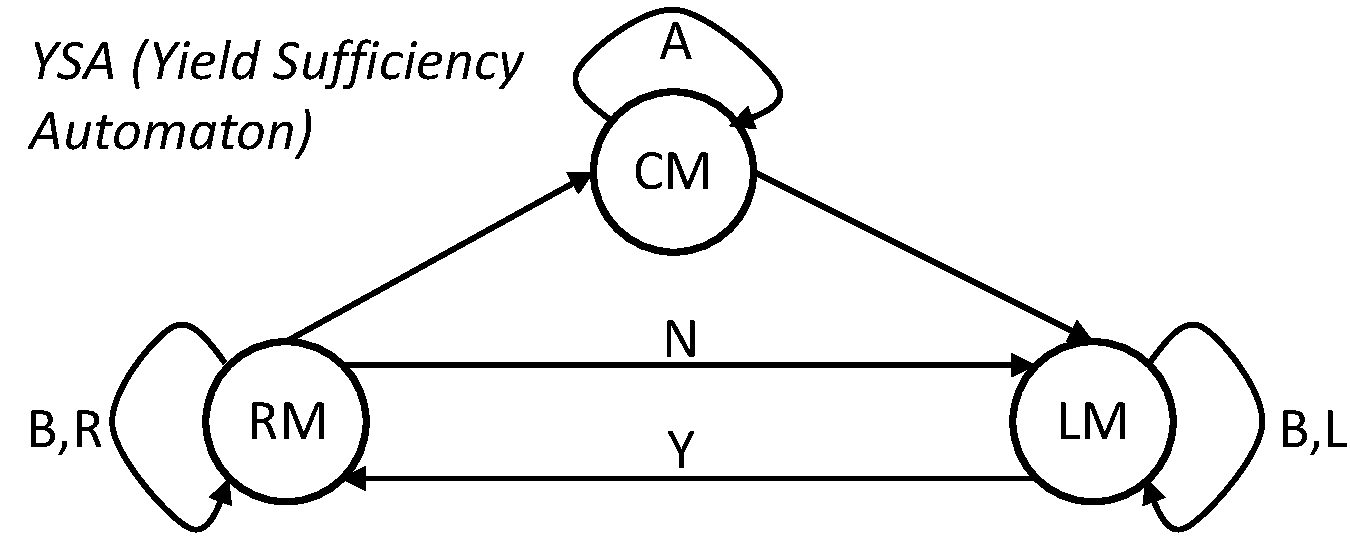
\includegraphics[scale=0.35]{YieldTypeCheckingAutomaton.pdf}
\caption{Specification for yield sufficiency}
\label{fig:YieldTypeCheckingAutomaton}
\end{figure}

\begin{figure*}
\scriptsize{
\medskip
%%%%%%%%%%%%%%%%%%%%
$
\inferrule
{
}
{\Refines;\actions \jy \skipstmt : (x, x)}
\;(\textsc{Skip})
$
\medskip
%%%%%%%%%%%%%%%%%%%%
$
\inferrule
{
}
{\Refines;\actions \jy \assert{\locExpr} : (x, x)}
\;(\textsc{Assert})
$
\medskip
%%%%%%%%%%%%%%%%%%%%
$
\inferrule
{
}
{\Refines;\actions \jy \yield{e,\lins} : (x, \RM)}
\;(\textsc{Yield})
$
\medskip
%%%%%%%%%%%%%%%%%%%%
$
\inferrule
{
P \not \in \dom(\Refines)
}
{\Refines;\actions \jy \call{P} : (x, \RM)}
\;(\textsc{Call})
$
\medskip
%%%%%%%%%%%%%%%%%%%%
$
\inferrule
{
P \in \dom(\Refines) \\ \actions(\Refines(P)) = (\rho, \alpha, B)
}
{\Refines;\actions \jy \call{P} : (x, x)}
\;(\textsc{BothMover})
$
\medskip
%%%%%%%%%%%%%%%%%%%%
$
\inferrule
{
P \in \dom(\Refines) \\ \actions(\Refines(P)) = (\rho, \alpha, R)
}
{\Refines;\actions \jy \call{P} : (\RM, \RM)}
\;(\textsc{RightMover})
$
\medskip
%%%%%%%%%%%%%%%%%%%%
$
\inferrule
{
P \in \dom(\Refines) \\ \actions(\Refines(P)) = (\rho, \alpha, L)
}
{\Refines;\actions \jy \call{P} : (x, \LM)}
\;(\textsc{LeftMover})
$
\medskip
%%%%%%%%%%%%%%%%%%%%
$
\inferrule
{
P \in \dom(\Refines) \\ \actions(\Refines(P)) = (\rho, \alpha, N)
}
{\Refines;\actions \jy \call{P} : (\RM, \LM)}
\;(\textsc{NonMover})
$
\medskip
%%%%%%%%%%%%%%%%%%%%
$
\inferrule
{
}
{\Refines;\actions \jy \async{P} : (x, \LM)}
\;(\textsc{Async})
$
\medskip
%%%%%%%%%%%%%%%%%%%%
$
\inferrule
{
x \in \{\RM,\CM\}
}
{\Refines;\actions \jy \ablock{e,\lins}{s} : (x, \CM)}
\;(\textsc{Ablock})
$
\medskip
%%%%%%%%%%%%%%%%%%%%
$
\inferrule
{
\Refines;\actions \jy \StmtStack : (x, y) \\ \Refines;\actions \jy s : (y, z)
}
{\Refines;\actions \jy \StmtStack;s : (x, z)}
\;(\textsc{Seq})
$
\medskip
%%%%%%%%%%%%%%%%%%%%
$
\inferrule
{
\Refines;\actions \jy s_1 : (x, y) \\ \Refines;\actions \jy s_2 : (x, y)
}
{\Refines;\actions \jy \ite{\locExpr}{s_1}{s_2} : (x, y)}
\;(\textsc{Ite})
$
\medskip
%%%%%%%%%%%%%%%%%%%%
$
\inferrule
{
\Refines;\actions \jy s : (x, x)
}
{\Refines;\actions \jy \while{e,\alpha}{\locExpr}{s} : (x, x)}
\;(\textsc{While})
$
\medskip
%%%%%%%%%%%%%%%%%%%%
$
\inferrule
{
\procs(P) = (\phi, \mods, \psi, \stmt) \\
\Refines;\actions \jy \stmt : (x, y)
}
{
\Refines;\actions \jy P
}
\;(\textsc{Procedure})
$
\medskip
%%%%%%%%%%%%%%%%%%%%
$
\inferrule
{
\Refines;\actions \jy \StmtStack : (x,y)
}
{
\Refines;\actions \jy (\varsL,\StmtStack) : (x,y)
}
\;(\textsc{Stack})
$
\medskip
%%%%%%%%%%%%%%%%%%%%
$
\inferrule
{
T = (\varsTL, (\varsL, \StmtStack)) \\
\Refines;\actions \jy (\varsL, \StmtStack) : (x, y)
}
{
\Refines;\actions \jy T
}
\;(\textsc{Thread})
$
\medskip
%%%%%%%%%%%%%%%%%%%%
$
\inferrule
{
\forall P \in \ProcName \setminus \dom(\Refines).\ \Refines;\actions \jy P \\\\
\forall 1 \le i \le n.\ \Refines;\actions \jy T_i
}
{
\Refines \jy (\procs, \actions, \ProcLins, \varsG, T_1 \ldots T_n)
}
\;(\textsc{Program})
$
\medskip
%%%%%%%%%%%%%%%%%%%%
}
\caption{Yield sufficiency rules}
\label{fig:yield-sufficiency}
\end{figure*}

\subsection{Program refinement}

\begin{figure*}
\scriptsize{
\medskip
%%%%%%%%%%%%%%%%%%%%
$
\inferrule
{
}
{\Refines;\RemovedActions \vdash \skipstmt \leadsto \skipstmt}
\;(\textsc{Skip})
$
\medskip
%%%%%%%%%%%%%%%%%%%%
$
\inferrule
{
}
{\Refines;\RemovedActions \vdash \assert{\locExpr} \leadsto \assert{\locExpr}}
\;(\textsc{Assert})
$
\medskip
%%%%%%%%%%%%%%%%%%%%
$
\inferrule
{
}
{\Refines;\RemovedActions \vdash \yield{e,\lins} \leadsto \yield{e,\lins}}
\;(\textsc{Yield})
$
\medskip
%%%%%%%%%%%%%%%%%%%%
$
\inferrule
{
A \not \in \RemovedActions
}
{\Refines;\RemovedActions \vdash \call{A} \leadsto \call{A}}
\;(\textsc{Atomic})
$
\medskip
%%%%%%%%%%%%%%%%%%%%
$
\inferrule
{
\Refines;\RemovedActions \vdash s \leadsto s'
}
{
\Refines;\RemovedActions \vdash \ablock{e,\lins}{s} \leadsto s'
}
\;(\textsc{Ablock-Elim})
$
\medskip
%%%%%%%%%%%%%%%%%%%%
$
\inferrule
{
\Refines;\RemovedActions \vdash s \leadsto s'
}
{
\Refines;\RemovedActions \vdash s \leadsto \ablock{e,\lins}{s'}
}
\;(\textsc{Ablock-Intro})
$
\medskip
%%%%%%%%%%%%%%%%%%%%
$
\inferrule
{
P \in \dom(\Refines)
}
{
\Refines;\RemovedActions \vdash \call{P} \leadsto \call{\Refines(P)}
}
\;(\textsc{Proc1})
$
\medskip
%%%%%%%%%%%%%%%%%%%%
$
\inferrule
{
P \not\in \dom(\Refines)
}
{
\Refines;\RemovedActions \vdash \call{P} \leadsto \call{P}
}
\;(\textsc{Proc2})
$
\medskip
%%%%%%%%%%%%%%%%%%%%
$
\inferrule
{
}
{
\Refines;\RemovedActions \vdash \async{P} \leadsto \async{P}
}
\;(\textsc{Async})
$
\medskip
%%%%%%%%%%%%%%%%%%%%
$
\inferrule
{
\Refines;\RemovedActions \vdash \StmtStack \leadsto \StmtStack'
}
{
\Refines;\RemovedActions \vdash (\varsL,\StmtStack) \leadsto (\varsL,\StmtStack')
}
\;(\textsc{Stack})
$
\medskip
%%%%%%%%%%%%%%%%%%%%
$
\inferrule
{
\Refines;\RemovedActions \vdash \StmtStack \leadsto \StmtStack' \\
\Refines;\RemovedActions \vdash \stmt \leadsto \stmt'
}
{
\Refines;\RemovedActions \vdash \StmtStack;\stmt \leadsto \StmtStack';\stmt'
}
\;(\textsc{Seq})
$
\medskip
%%%%%%%%%%%%%%%%%%%%
$
\inferrule
{
\Refines;\RemovedActions \vdash s_1 \leadsto s_1' \\
\Refines;\RemovedActions \vdash s_2 \leadsto s_2'
}
{
\Refines;\RemovedActions \vdash \ite{\locExpr}{s_1}{s_2} \leadsto \ite{\locExpr}{s_1'}{s_2'}
}
\;(\textsc{Ite})
$
\medskip
%%%%%%%%%%%%%%%%%%%%
$
\inferrule
{
\Refines;\RemovedActions \vdash s \leadsto s'
}
{
\Refines;\RemovedActions \vdash \while{e,\alpha}{\locExpr}{s} \leadsto \while{e,\alpha}{\locExpr}{s'}
}
\;(\textsc{While})
$
\medskip
%%%%%%%%%%%%%%%%%%%%
$
\inferrule
{
\Refines;\RemovedActions \vdash \stmt \leadsto \stmt'
}
{
\Refines;\RemovedActions \vdash (\phi,\mods,\psi,\stmt) \leadsto (\phi',\mods',\psi',\stmt')
}
\;(\textsc{Procedure})
$
\medskip
%%%%%%%%%%%%%%%%%%%%
$
\inferrule
{
\accessVars(\rho) \cap \Local = \emptyset \\
\alpha = ((\exists \mathit{old}(\Local), \Local.\ \alpha) \wedge \Same(\Local)) \\
}
{
\Refines;\RemovedActions \vdash (\rho,\alpha,m) \leadsto (\rho,\alpha,m)
}
\;(\textsc{Action})
$
\medskip
%%%%%%%%%%%%%%%%%%%%
$
\inferrule
{
\Refines;\RemovedActions \vdash \StmtStack \leadsto \StmtStack' \\
}
{
\Refines;\RemovedActions \vdash (\varsTL, (\varsL, \StmtStack)) \leadsto (\varsTL, (\varsL, \StmtStack')) \\
}
\;(\textsc{Thread})
$
\medskip
%%%%%%%%%%%%%%%%%%%%
$
\inferrule
{
\Prog = (\procs, \actions, \ProcLins, \varsG, T_1 \ldots T_n) \\
\Prog' = (\procs', \actions', \ProcLins', \varsG, T_1' \ldots T_n') \\
\forall 1 \le i \le n.\ \Refines;\RemovedActions \vdash T_i \leadsto T_i' \\
\forall A \not\in \RemovedActions.\ \actions(A) = \actions'(A) \\
\forall A \in \range(\Refines).\ \Refines;\RemovedActions \vdash \actions(A) \leadsto \actions(A) \\
\forall P \not\in \dom(\Refines).\ \Refines;\RemovedActions \vdash \procs(P) \leadsto \procs'(P) \\
\forall P \in \dom(\Refines).\ \ProcLins(P) = \ProcLins(\Refines(P)) \\
}
{
\Refines;\RemovedActions \vdash \Prog \leadsto \Prog'
}
\;(\textsc{Program})
$
\medskip
%%%%%%%%%%%%%%%%%%%%
}
\caption{Program refinement}
\label{fig:program-refinement}
\end{figure*}

\subsection{Soundness}

\begin{theorem}
Let $\Prog$ and $\Prog'$ be two programs.
Let $\Refines \in \ProcName \pf \ActionName$ be a partial function from procedure names to action names.
Let $\RemovedActions \in 2^{\ActionName}$ be a set of action names.
Suppose the following conditions are satisfied:
\begin{enumerate}
\item
$\vdash \Prog$ and $\vdash \Prog'$ and $\Refines;\RemovedActions \vdash \Prog \leadsto \Prog'$.
\item 
All finite executions of $\Prog'$ are safe.
\item
All infinite executions of $\Prog'$ are responsive.
\item
$\CommutativitySafe(\Prog)$.
\item
$\InterferenceFree(\Prog,\Refines)$.
\item
$\Refines \jp Prog$ and $\Refines \jr Prog$ and $\Refines \jy Prog$.
\end{enumerate}
Then all finite executions of $\Prog$ are safe.
\end{theorem}

\subsection{Responsiveness}

\[
\inferrule
{
\procs;\actions;\RefinementAny;\mods \jp \FH{e \wedge \locExpr}{s}{e} \\ e \wedge \locExpr \Rightarrow f \geq 0 \\ s \preceq (old(e \wedge \locExpr) \Rightarrow \mathit{old}(f) > f)
}
{\procs;\actions;\RefinementAny;\mods \jp \FH{e}{\while{e,\alpha,f}{\locExpr}{s}}{e \wedge \neg \locExpr}}
\;(\textsc{While})
\]


\section{A concurrent garbage collector}
\label{sec:gc}
\begin{figure*}
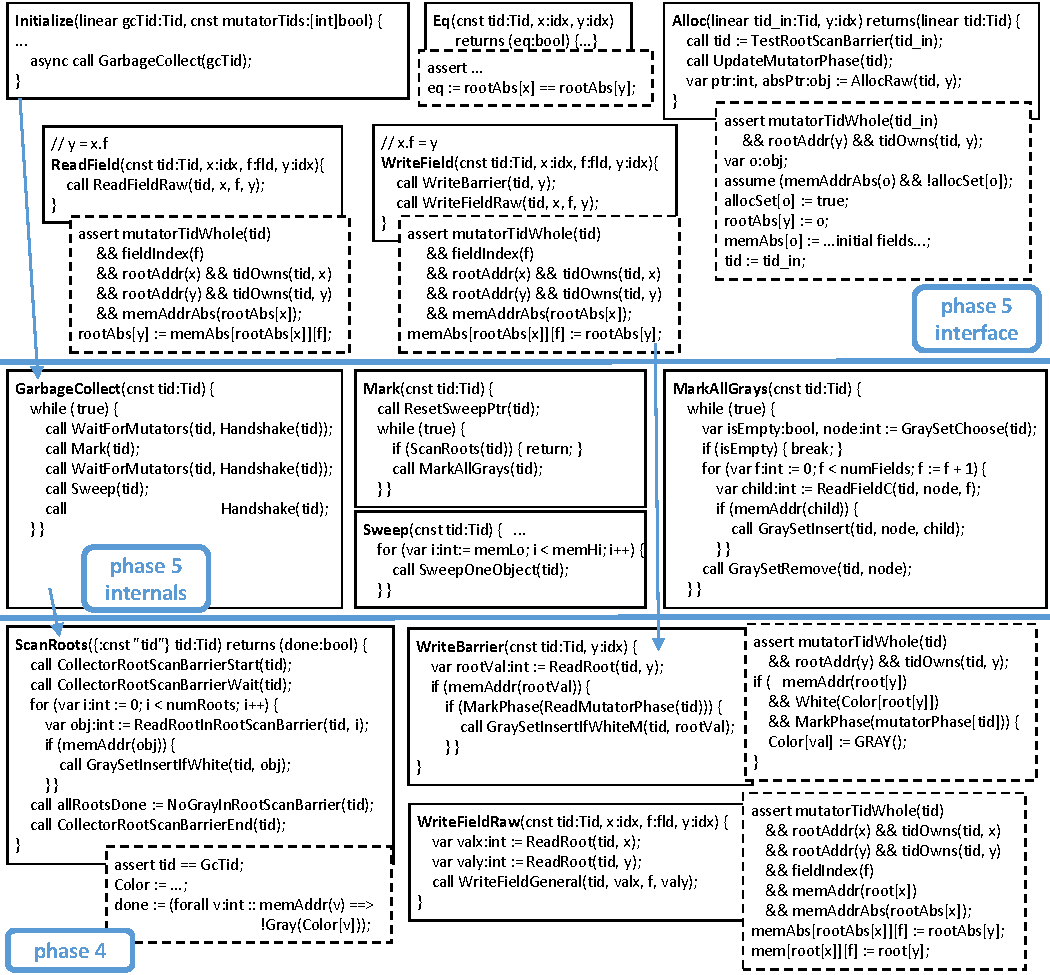
\includegraphics[scale=1.0]{VerifiedGC.pdf}
\caption{Verified garbage collector phases 5, 6 (pseudocode excerpts in solid boxes; atomic action specs in dashed boxes)}
\label{fig:VerifiedGC}
\end{figure*}

We demonstrate the verification methodology and tool on a realistic modern concurrent garbage collector algorithm.
Our algorithm builds on the concurrent collector of Dijkstra et. al.~\cite{dijk78}.
Dijkstra's collector is attractive for verification because it maintains a simple three-color invariant
on the heap objects (contrasting with snapshot-oriented collectors~\cite{doli93,doli94,doma00,azat03},
whose three-color invariants are more subtle).
By itself, though, Dijkstra's collector is not a modern or performant collector.
First, it becomes incorrect in the presence of more than one program thread (mutator).
Second, it requires that the write-barrier be run not only on updates of heap pointers,
but also on modifications of root pointers, i.e., on modifications of the runtime stacks and the registers;
modern high-performance collectors avoid this overhead.

Therefore, our algorithm (shown inside the solid boxes in Figure~\ref{fig:VerifiedGC}) extends and modifies Dijkstra's collector
to make it work with parallel programs and to not require a write-barrier on root modifications.
Like Dijkstra's collector, our algorithm first {\em marks} all objects reachable from roots (registers and stacks),
shown in Figure~\ref{fig:VerifiedGC}'s Mark procedure, and then sweeps away all unreached objects,
shown in Figure~\ref{fig:VerifiedGC}'s Sweep procedure.
As in Dijkstra's collector, our algorithm employs a tri-color abstraction to describe the trace of the reachable objects.
Objects are said to be {\em white} if the collector has not seen them yet during the trace.
Objects that the collector encounters become gray and remain gray until the collector scans their children.
Once all the children of an object are noted (meaning that none of them are white), the object becomes black.
The collector works by choosing a node from the set of gray objects (GraySetChoose in Figure~\ref{fig:VerifiedGC}, called from MarkAllGrays),
{\em shading} all its white children to gray (GraySetInsert), and then removing the object from the gray set by making the object black (GraySetRemove).
The shading operation grays a node if it is white, and does noting otherwise.
The trace terminates when all roots point to black objects (according to ScanRoots)
and there are no more gray objects in the heap (according to IsGraySetEmpty, called by ScanRoots).
Termination is guaranteed because objects can only get darker.
Correctness is guaranteed using an invariant that black objects never point to white pointer during the trace
(black objects can only point to gray objects or black objects).
At the end of the trace, objects pointed by the roots must be black, and since no gray objects remain,
black objects only point to black objects,
so the entire set of objects reachable from the roots must be black.

Concurrent mutator operations on objects (ReadField and WriteField in Figure~\ref{fig:VerifiedGC})
could potentially break the no-black-to-white invariant,
because a mutator's WriteField operation could potentially redirect a pointer of a black object to point to a white object.
Therefore, coordination between the program and the concurrent collector is required:
Before each raw pointer update (WriteFieldRaw), the WriteField procedure executes a {\em write-barrier} (WriteBarrier).
Before pointer field $x.f$ is set to reference an object $y$,
WriteBarrier shades $y$, ensuring that even if $x$ is black, a pointer from $x$ to $y$
will not violate the no-white-to-black invariant.

The write barrier should shade objects only while the collector is in its mark phase,
not when the collector is sweeping or is idle, and the collector may only switch between phases (mark, sweep, or idle)
when no mutator is in the middle of a WriteField or Alloc operation.
To achieve this (and thereby support correct and efficient support for multiple mutator threads),
we extend Dijkstra's collector with explicit tracking of phases, via a handshaking mechanism~\cite{doli93,doli94}.
A shared variable, collectorPhase, contains the current collector phase.
The collector initiates a handshake by incrementing collectorPhase (in Handshake, called by GarbageCollect).
Each mutator thread keeps cached copy of collectorPhase, and periodically checks to see if
the cached copy mismatches the current collectorPhase, and if so, updates the cached copy
with the most recent value
(in our algorithm, a mutator's call to the allocator, Alloc, checks this in UpdateMutatorPhase,
but the exact location of the check is not critical to correctness).
The GarbageCollector waits until all cached copies equal collectorPhase (WaitForMutators in GarbageCollect),
and then executes a phase (Mark, Sweep, or, for the idle phase, nothing).
Note that each mutator thread can read its own cached phase without acquiring a lock (ReadMutatorPhase in WriteBarrier),
leading to efficient WriteBarrier performance.

Dijkstra's collector requires a write barrier on modifications to roots as well as modifications to objects.
To eliminate this overhead, our algorithm pauses all threads while scanning the roots.
Similar to the implementation of handshaking, ScanRoots signals to the mutator threads that a root scan
is about to begin (CollectorRootScanBarrierStart), waits (CollectorRootScanBarrierWait) for the
mutators to respond and pause (TestRootScanBarrier), scans the roots while the mutators are paused,
and then wakes up the mutators (CollectorRootScanBarrierEnd).
At the end of the scan (before the mutators reawaken), all roots point to gray or black objects.
If no gray objects remain (IsGraySetEmpty), then all roots point to black objects, and the marking is complete.
Otherwise, we continue the collection by shading all objects reachable by the roots and tracing from them again.
In a worst-case theoretical scenario we may need to run many root scans and discover more and more white root descendants to trace each time. 
But in practice we usually finish after a small number of scans,
so we obtain correctness and termination in all scenarios and we obtain good performance in real-world scenarios. 




\subsection{Collector Verification in Boogie}

We have implemented and verified our algorithm in Boogie,
including initialization (Initialize), the GC (GarbageCollect), the allocator (Alloc),
and the mutator operations (ReadField, WriteField, and Eq, which tests for pointer equality),
and all the lower-level operations required to implement them (some of which appear
in Figure~\ref{fig:VerifiedGC}, but most of which are omitted from the figure to save space).
To make the verification as realistic as possible,
our Boogie code implements everything in terms of individual CPU operations,
such as load, store, atomic increment/decrement, and CAS (compare-and-swap);
in contrast to some previous work~\cite{gont96},
we do not assume any built-in higher-level operations.
To ease verification, we make some simplifications:
we use a naive allocator (sequential search for free space),
we assume a sequentially consistent memory model,
and we assume that all objects have the same number of fields.
(Except for the assumption of sequential consistency, none of these substantially alter the nature of the proof.)
Overall, our implementation consists of about 2100 lines of Boogie code,
and it takes Boogie/Z3 about 80 minutes to verify.

Our verification takes advantage of all three techniques in \civl: refinement, Owicki-Gries/Rely-Guarantee, and linearity.
Refinement gives us extremely simple high-level action specifications for Initialize, ReadField, WriteField, Eq, and Alloc,
shown in their entirety in Figure~\ref{fig:VerifiedGC}'s dashed boxes.
(Initialize and GarbageCollect have empty actions; the GarbageCollector itself is just an internal implementation detail inside Initialize,
which serves only to set up the global GC invariant needed by the other high-level actions.)
Crucially, ReadField, WriteField, Eq, and Alloc appear atomic to mutators, even though internally,
WriteField and Alloc involve many interleaved operations on shared GC data structures.
Figure~\ref{fig:VerifiedGC} shows only shows phases 5 and 6, the two most abstract phases of refinement;
phases 1-4 fill in the implementation details,
such as implementing the set of gray objects as an explicit stack (an array of elements with a pointer to the stack top, in phase 4),
handshaking (phase 3), locks (phase 2), and wrapping the primitive CPU operations in left/right/non-moving atomic actions (phase 1).
Ultimately, the phases are built on trusted CPU-level atomic actions, such as reading and writing roots directly:

\begin{verbatim}
procedure PrimitiveWriteRoot(i:idx, v:int);
ensures{:atomic} [assert rootAddr(i); root[i] := v;]

procedure PrimitiveReadRoot(i:idx) returns (v:int);
ensures{:atomic} [assert rootAddr(i); v := root[i];]
\end{verbatim}

We write the highest-level action specifications in terms of an abstract view of memory,
as in earlier work on sequential garbage collector verification~\cite{mccr07,hawb09}.
(Abstract memory is infinite and eternal: once allocated, an abstract object lives forever.
Deallocation is an underlying implementation detail, not exposed in the abstract interface.)
Our abstract view describes a machine as consisting of just three variables:
abstract memory memAbs:[obj][fld]obj, mapping object identifiers and fields to other objects,
abstract root values rootAbs:[idx]obj, mapping root names to objects, and
allocSet:[obj]bool, the set of objects allocated so far.
At this high layer of abstraction, we use Boogie's hiding to hide all other variables
(such as the concrete root set, ``root'', the concrete memory, ``mem'', and the colors, ``Color'', used by lower-level procedures).

All operations are relative to root names of type idx.
ReadField, for example, reads an object field from an object pointed to by root x into a root y.
The predicates rootAddr and tidOwns establish that x and y are valid root names, owned by a particular mutator tid.
(We assume that each root is private to a single mutator stack or register file;
sharing between mutator threads takes place through shared pointers to objects.)
The predicates fieldIndex(f) and memAddrAbs(o) establish that x.f is a valid field of a valid object.
Allocation establishes memAddrAbs(o) for newly allocated objects so that they may be used by subsequent ReadField and WriteField operations.
It also establishes o's unique identity by ensuring that it did not previously belong to the allocated object set.

In addition to atomic action specifications, the verification establishes invariants using Owicki-Gries/Rely-Guarantee reasoning
(omitted from Figure~\ref{fig:VerifiedGC} to save space).
For example, Initialize establishes a global mapping toAbs:[int]obj from physical memory mem and abstract memory memAbs,

\begin{verbatim}
(forall x:int, f:fld ::
   memAddr(x) && toAbs[x] != nil && fieldIndex(f)
  ==> toAbs[mem[x][f]] == memAbs[toAbs[x]][f])
\end{verbatim}

and Mark maintains the no-black-to-white invariant:

\begin{verbatim}
(forall x:int, f:fld ::
  memAddr(x) && Black(Color[x]) && fieldIndex(f)
             && memAddr(mem[x][f]) ==>
  Gray(Color[mem[x][f]]) || Black(Color[mem[x][f]]))
\end{verbatim}

Finally, linearity plays a key role in establishing mutual exclusion.
The GC thread has its own thread id gcTid, and each mutator has its own thread id.
The Initialize procedure consumes gcTid (written here as ``consume'')
and borrows all the mutator thread ids (written as ``linear'', as in Section~\ref{sec:overview}),
so that it's clear that no other concurrent actions are allowed during initialization.
This allows all the internal initialization actions to be movers, without requiring any explicit locking.
Initialize must consume gcTid because it passes gcTid to the newly spawned GarbageCollector thread;
since gcTid is consumed, it's impossible to call Initialize twice in an attempt to spawn two parallel GC threads
(which naturally expresses how the algorithm is only safe for a single GC thread).

Because \civl's linearity is based on sets of values,
we can represent thread identifiers as sets that can be subdivided into subsets
(similar to how fractional permissions may be divided into fractions).
During root scanning, each mutator thread places a non-empty fraction of its thread id in a global variable,
and extracts the fraction from the global variable after root scanning completes;
the collector maintains the invariant that the global variable contains non-empty fractions from all the mutators during root scanning.
Thus, during root scanning, \civl's rules for linearity prove that no interference is possible
between the collector and any mutator operations that require the whole mutator thread id
(``mutatorTidWhole'', used in Figure~\ref{fig:VerifiedGC}'s ReadField, WriteField, Alloc,
and most other mutator operations).


\section{Related work}
\label{sec:related}

\section{Related work}
\label{sec:related}

Our work is the first to provide a tool and theory to support automated,
modular whole-program refinement through multiple layers, as distinct from existing work on
single-layer atomicity refinement between procedure implementations and
specifications. 
\civl combines a number of techniques in a novel manner to 
decompose the refinement task following the syntactic structure of a
program. Below, we first contrast \civl with refinement
verification techniques, and then with tools and
techniques for reasoning about concurrent programs in general. 

\subsection{Refinement-oriented verification}
Atomic action specifications have been explored by the
\calvin~\cite{FlanaganFQS05,FreundQ04} verifier. 
\civl carries out refinement verification on a procedure body
with cooperative semantics as enabled by movers types and reduction.
\calvin attempts to verify refinement directly on the preemptive
semantics, making only limited use of movers at the lowest-level
representation. 
\calvin, unlike does not support location invariants and linear
variables but incorporates rely-guarantee reasoning. 
\civl supports both location
invariants or rely-guarantee reasoning, and either technique can be
used to prove non-interference.
However, in certain cases, rely-guarantee reasoning
requires use of auxiliary (shared) variables and makes interactive
proofs difficult as was the case in our GC proof. 

\QED~\cite{ElmasQT09} is a simplifier for concurrent programs and is close in spirit to the 
refinement-oriented approach of \civl.
A key distinction between \civl and \QED is the fact that a proof step in \QED is a small rewrite in the concurrent program
that must be justified by potentially expensive reduction and invariant reasoning.
In \QED, procedures can be proven atomic only one procedure at a time, and only by
transforming their bodies by reduction to be yield free. 
The number of small proof steps directly affect both programmer
and computer effort. 
By contrast, \civl supports large proof steps, in each of which the bodies of several procedures
are automatically replaced by atomic actions, thereby lowering the cost of both interaction and automation.
The non-interference reasoning in \QED is even more limited than \calvin.
\QED supports only global invariants and does not support rely-guarantee reasoning or linear variables.

Liang et al.~\cite{LiangRGSim} present a method for verifying that procedure
bodies refine atomic specifications
The key verification approach is
rely-guarantee reasoning and the refinement (simulation) relation between
a procedure and its specification is constrained so it is preserved under
parallel composition. 
No tool support is provided. 
Authors present a (paper) GC proof, which is limited in scope compared
to ours, as their proof corresponds to a few layers of our proof. In particular,
the GC is not refined down to individual atomic memory accesses. 
Since this work uses different languages to describe the high-level
and low-level programs, it is not immediately possible to carry out a
multi-level stepwise refinement proof. 

Turon and Wand~\cite{TuronM11} use ownership disciplines and
separation logic to verify refinement of atomic specifications by 
concurrent data structure implementations. 
Rely-guarantee reasoning is
supported to provide compositionality and non-interference
arguments. 
This work targets a single refinement step between atomic
specifications for methods and their implementations. 
No tool support for this verification method is provided. 

Verifying linearizability of concurrent data structures (see, e.g.,
\cite{tacasLin,aliLin}) can be viewed as an instance of one-level of
refinement in our setting. 
\civl can be used for mechanical
verification of linearizability, as we did for the Treiber stack. 
Tools and techniques specific to verifying linearizability
cannot be easily generalized for stepwise refinement proofs
through multiple levels. 

Refinement proofs
between implementations and specifications of protocols have been
investigated using the TLA+~\cite{Lamport2004} specification
language. 
Compositional refinement proofs~\cite{AbadiAssumeGuarantee} have
been investigated in this context. 
Modular refinement proofs for hardware systems have been investigated extensively
(e.g.,~\cite{Henzinger1999,Eiriksson2000}) using the SMV~\cite{McMillan00} and Mocha~\cite{AlurHMQRT98} 
model checking tools.
To verify a concurrent, shared-memory program using such tools, one must encode
the program semantics as a state-transition system and express
verification goals in terms of this system. 
For concurrent, shared-memory
software, \civl enables reasoning on the structured, imperative
multithreaded program text rather than a logic description of the
program's state-transition relation. 
 

\subsection{Reasoning about concurrency}
In this section, we discuss foundational techniques
for combating the complexity of concurrent program verification. 
\civl and refinement techniques discussed in the previous
section have common ideas with tools and formalisms
discussed in this section, however, the latter primarily target verification of a {\em single} program rather than refinement. 
Refinement in \civl is orthogonal to these techniques, which can be aided by \civl's 
ability to connect a complex concurrent program to a simpler abstraction.

VCC~\cite{VCC} is a tool for verifying concurrent C programs.  
Chalice~\cite{LM09} is a language and modular verification tool for concurrent programs. 
VCC does not support refinement and Chalice does so only for sequential programs.  
VCC and Chalice base their invariant reasoning on objects, object ownership, and type invariants. 
Invariant reasoning in \civl is more primitive and based on predicates in yield statements. 
Although the approach in VCC and Chalice is more convenient when applicable, \civl's approach is more flexible. 
VCC and Chalice can reason sequentially about objects exclusively owned by a thread;
\civl accomplishes the same using linear variables.
Neither VCC nor Chalice support movers and reduction reasoning.

Concurrent separation logic~\cite{OHearn07} reasons about concurrency without 
explicitly checking for non-interference between threads. 
Recently, tools based on this logic that blend in explicit
non-interference reasoning (but without support for reduction and mover reasoning) have been developed~\cite{SAGL,RGSep}. 
\civl's combination of interference checking and linear variables is
an extreme example of this trend, is very general and technique-agnostic. 
We supply very primitive abstractions and let programmers mix and
match these abstractions freely to encode the non-interference reasoning style of their choice. 





\bibliographystyle{abbrv}
\bibliography{paper}

\newpage

% moved to supplement.tex:
%\appendix
%\section{Operational semantics}
\label{sec:operational-semantics}

\begin{figure}
\scriptsize{
\medskip
%%%%%%%%%%%%%%%%%%%%
$
\inferrule
{
\ProgCtxt[\varsG][\varsTL][\varsL][s] = (\_, \actions, \_, \_, \_) \\
\actions \vdash (\MakeStore{\varsG}{\varsTL}{\varsL}, s) \trans (\MakeStore{\varsG'}{\varsTL'}{\varsL'}, s')
}
{\ProgCtxt[\varsG][\varsTL][\varsL][s] \trans \ProgCtxt[\varsG'][\varsTL'][\varsL'][s']}
\;(\textsc{Step})
$
\medskip
%%%%%%%%%%%%%%%%%%%%
$
\inferrule
{
\ProgCtxt[\varsG][\varsTL][\varsL][s] = (\_, \actions, \_, \_, \_) \\
\actions \vdash (\MakeStore{\varsG}{\varsTL}{\varsL}, s) \fails
}
{\ProgCtxt[\varsG][\varsTL][\varsL][s]) \fails}
\;(\textsc{Fail})
$
\medskip
%%%%%%%%%%%%%%%%%%%%
$
\inferrule
{
\procs(P) = (\phi, \mods, \psi,\stmt) \\
\ProcLins(P) = (\lins, \lins') \\
T' = (\varsTL, (\varsL, \yield{\phi,\lins};\stmt)) \\
\TS = \ThreadCtxt[\varsTL][\varsL][\async{P}] \\
\TS' = \ThreadCtxt[\varsTL][\varsL][\skipstmt]
}
{
(\procs, \actions, \ProcLins, \varsG, \TS)
\trans
(\procs, \actions, \ProcLins, \varsG, \TS' \cdot T')
}
\;(\textsc{Async})
$
\medskip
%%%%%%%%%%%%%%%%%%%%
$
\inferrule
{
T = (\varsTL, (\varsL,\skipstmt)) 
}
{(\procs, \actions, \ProcLins, \varsG, \YieldingThreads \cdot T \cdot \YieldingThreads') \trans (\procs, \actions, \ProcLins, \varsG, \YieldingThreads \cdot \YieldingThreads')}
\;(\textsc{End})
$
\medskip
%%%%%%%%%%%%%%%%%%%%
$
\inferrule
{
\procs(P) = (\phi, \mods, \psi,\stmt) \\
\ProcLins(P) = (\lins, \lins') \\
\StmtStack = \yield{\phi,\lins};\stmt;\yield{\psi,\lins'}
}
{\ProgCtxt[\varsG][\varsTL][\varsL][\call{P}] \trans \ProgCtxt[\varsG][\varsTL][\varsL][\Frame{L}{\StmtStack}]}
\;{(\textsc{Call})}
$
\medskip
%%%%%%%%%%%%%%%%%%%%
$
\inferrule
{
\\
}
{\ProgCtxt[\varsG][\varsTL][\varsL][\Frame{\varsL'}{\skipstmt}] \trans \ProgCtxt[\varsG][\varsTL][\varsL][\skipstmt]}
\;{(\textsc{Return})}
$
%%%%%%%%%%%%%%%%%%%%
}
\caption{Operational semantics for program}
\label{fig:operational-semantics1}
\end{figure}


\begin{figure}
\scriptsize{
\medskip
%%%%%%%%%%%%%%%%%%%%
$
\inferrule
{
\vars = \MakeStore{\varsG}{\varsTL}{\varsL} \\
\varsL \in \locExpr
}
{\actions \vdash (\vars, \assert{\locExpr}) \trans (\vars, \skipstmt)}
\;{(\textsc{Assert-True})}
$
\medskip
%%%%%%%%%%%%%%%%%%%%
$
\inferrule
{
\vars = \MakeStore{\varsG}{\varsTL}{\varsL} \\
\varsL \not \in \locExpr
}
{\actions \vdash (\vars, \assert{\locExpr}) \fails}
\;{(\textsc{Assert-False})}
$
\medskip\\
%%%%%%%%%%%%%%%%%%%%
$
\inferrule
{
\actions(A) = (\rho, \alpha, m) \\
(\vars, \vars') \in \alpha \\
}
{
\actions \vdash (\vars, \call{A}) \trans (\vars',\skipstmt)
}
\;{(\textsc{Atomic})}
$
\medskip
%%%%%%%%%%%%%%%%%%%%
$
\inferrule
{
\\
}
{\actions \vdash (\vars, \yield{e,\lins}) \trans (\vars, \skipstmt)}
\;{(\textsc{Yield})}
$
\medskip
%%%%%%%%%%%%%%%%%%%%
$
\inferrule
{
}
{\actions \vdash (\vars, \ablock{e,\lins}{\stmt}) \trans (\vars, \stmt)}
\;{(\textsc{AtomicBlock})}
$
\medskip
%%%%%%%%%%%%%%%%%%%%
$
\inferrule
{
\\
}
{\actions \vdash (\vars, \skipstmt;\stmt) \trans (\vars, \stmt)}
\;{\;\;\;\;\;\;\;\;\;\;\;\;(\textsc{Seq})}
$
\medskip
%%%%%%%%%%%%%%%%%%%%
$
\inferrule
{
\vars = \MakeStore{\varsG}{\varsTL}{\varsL} \\
\varsL \not\in \locExpr
}
{\actions \vdash (\vars, \ite{\locExpr}{s_1}{s_2}) \trans (\vars, s_2)}
\;{(\textsc{If-False})}
$
\medskip
%%%%%%%%%%%%%%%%%%%%
$
\inferrule
{
\vars = \MakeStore{\varsG}{\varsTL}{\varsL} \\
\varsL \in \locExpr
}
{\actions \vdash (\vars, \ite{\locExpr}{s_1}{s_2}) \trans (\vars, s_1)}
\;{(\textsc{If-True})}
$
\medskip
%%%%%%%%%%%%%%%%%%%%
$
\inferrule
{
\vars = \MakeStore{\varsG}{\varsTL}{\varsL} \\
\varsL \not\in \locExpr \\
}
{\actions \vdash (\vars, \while{e,\alpha}{\locExpr}{s}) \trans (\vars, \skipstmt)}
\;{(\textsc{While-False})}
$
\medskip
%%%%%%%%%%%%%%%%%%%%
$
\inferrule
{
\vars = \MakeStore{\varsG}{\varsTL}{\varsL} \\
\varsL \in \locExpr \\
\stmt' = \while{e,\alpha}{\locExpr}{\stmt}
}
{\actions \vdash (\vars, \stmt') \trans (\vars, \stmt;\stmt')}
\;{(\textsc{While-True})}
$
%%%%%%%%%%%%%%%%%%%%
}
\caption{Operational semantics for statement}
\label{fig:operational-semantics2}
\end{figure}

Figures~\ref{fig:operational-semantics1} and~\ref{fig:operational-semantics2} together present the operational semantics as a relation $\trans$ between a pair of programs.
These figures use the notation $\MakeStore{\varsG}{\varsTL}{\varsL}$ to denote the concatenation of the stores $\varsG$, $\varsTL$, and $\varsL$.
Rule \textsc{Step} in Figure~\ref{fig:operational-semantics2} allows the program $\ProgCtxt[\varsG][\varsTL][\varsL][\stmt]$ to move 
to $\ProgCtxt[\varsG'][\varsTL'][\varsL'][\stmt']$
if $(\MakeStore{\varsG}{\varsTL}{\varsL}, \stmt)$ can move to $(\MakeStore{\varsG'}{\varsTL'}{\varsL'}, \stmt)$ 
according to any rule in Figure~\ref{fig:operational-semantics2} except for rule \textsc{Assert-False}.
Similarly, rule~\textsc{Fail} allows $\ProgCtxt[\varsG][\varsTL][\varsL][\stmt]$ to fail if $(\MakeStore{\varsG}{\varsTL}{\varsL}, \stmt)$
fails according to rule \textsc{Assert-False}. 
The rules in  in Figure~\ref{fig:operational-semantics2} are straightforward.
The execution of primitive statements results in the store begin updated and the statement being rewritten to $\skipstmt$;
the rule \textsc{Seq} erases the $\skipstmt$ to move control to the next statement.

Rule \textsc{Async} describes the creation of a thread via $\async{P}$.  
There is an implicit yield at the beginning of the freshly-created thread.
The stable predicate and the linear permission associated with this yield are 
the precondition and the input linear permission of $P$.
The new thread is added to the sequence of threads in the program.
Since it is a yielding thread, the invariant that at most one thread is non-yielding is preserved.
Rule \textsc{End} describes the termination of a thread; the terminating thread is removed
from the sequence of threads in the program.
Rules \textsc{Call} and \textsc{Return} describe the call and return of a procedure via $\call{P}$.
There are implicit yields associated with the call and the return.
The stable predicates for the yields at call and return are the precondition and postcondition of $P$ respectively.
The linear permissions for the yields at call and return are the input and output linear permissions of $P$ respectively.


\section{Verification}
\label{sec:verification-appendix}

\begin{figure}
\scriptsize{
\medskip
%%%%%%%%%%%%%%%%%%%%
$
\inferrule
{
}
{\procs;\actions;\RefinementAny;\{\} \js \FH{\phi}{\skipstmt}{\phi}}
\;(\textsc{Skip})
$
\medskip\\
%%%%%%%%%%%%%%%%%%%%
$
\inferrule
{
}
{\procs;\actions;\RefinementInside;\{\} \js \FH{\phi \wedge \locExpr}{\assert{\locExpr}}{\phi}}
\;(\textsc{Assert1})
$
\medskip
%%%%%%%%%%%%%%%%%%%%
$
\inferrule
{
}
{\procs;\actions;\RefinementOutside;\{\} \js \FH{\phi}{\assert{\locExpr}}{\phi}}
\;(\textsc{Assert2})
$
\medskip
%%%%%%%%%%%%%%%%%%%%
$
\inferrule
{
}
{\procs;\actions;\RefinementAny;\{\} \js \FH{e}{\yield{e,\lins}}{e}}
\;(\textsc{Yield})
$
\medskip
%%%%%%%%%%%%%%%%%%%%
$
\inferrule
{
\actions(A) = (\rho, \alpha, m) \\ 
\mods \subseteq \ThreadLocal \\
\alpha \Rightarrow \Havoc(\Global \cup \mods \cup \Local) \\
\phi \Rightarrow \rho \\ 
\Unsat{\phi \circ \alpha \circ \neg \psi} \\
}
{\procs;\actions;\RefinementAny;\mods \js \FH{\phi}{\call{A}}{\psi}}
\;(\textsc{Atomic})
$
\medskip
%%%%%%%%%%%%%%%%%%%%
$
\inferrule
{
\procs(P) = (\phi, \mods, \psi, \stmt) \\ P \not \in \dom(\Refines)
}
{\procs;\actions;\RefinementAny;\mods \js \FH{\phi}{\call{P}}{\psi}}
\;(\textsc{Proc1})
$
\medskip
%%%%%%%%%%%%%%%%%%%%
$
\inferrule
{
\procs(P) = (\phi, \mods, \psi, \stmt) \\ P \in \dom(\Refines) \\\\ \procs;\actions;\RefinementAny;\mods \js \FH{\phi}{\call{\Refines(P)}}{\psi}
}
{\procs;\actions;\RefinementAny;\mods \js \FH{\phi}{\call{P}}{\psi}}
\;(\textsc{Proc2})
$
\medskip
%%%%%%%%%%%%%%%%%%%%
$
\inferrule
{
\procs(P) = (\phi, \mods, \psi, \stmt)
}
{\procs;\actions;\RefinementAny;\{\} \js \FH{\rho \wedge \phi}{\async{P}}{\rho}}
\;(\textsc{Async})
$
\medskip
%%%%%%%%%%%%%%%%%%%%
$
\inferrule
{
\procs;\actions;\RefinementAny;\mods \js \FH{\phi_1 \wedge e}{s}{\phi_2}
}
{\procs;\actions;\RefinementAny;\mods \js \FH{\phi_1 \wedge e}{\ablock{e,\lins}{s}}{\phi_2}}
\;(\textsc{Ablock})
$
\medskip
%%%%%%%%%%%%%%%%%%%%
$
\inferrule
{
\procs;\actions;\RefinementAny;\mods_1 \js \FH{\phi_1}{\StmtStack}{\phi_2} \\ 
\procs;\actions;\RefinementAny;\mods_2 \js \FH{\phi_2}{s}{\phi_3}
}
{\procs;\actions;\RefinementAny;\mods_1 \cup \mods_2 \js \FH{\phi_1}{\StmtStack;s}{\phi_3}}
\;(\textsc{Seq})
$
\medskip
%%%%%%%%%%%%%%%%%%%%
$
\inferrule
{
\procs;\actions;\RefinementAny;\mods_1 \js \FH{e \wedge \phi_1}{s_1}{\phi_2} \\ 
\procs;\actions;\RefinementAny;\mods_2 \js \FH{\neg e \wedge \phi_1}{s_2}{\phi_2}
}
{\procs;\actions;\RefinementAny;\mods_1 \cup \mods_2 \js \FH{\phi_1}{\ite{\locExpr}{s_1}{s_2}}{\phi_2}}
\;(\textsc{Ite})
$
\medskip
%%%%%%%%%%%%%%%%%%%%
$
\inferrule
{
\procs;\actions;\RefinementAny;\mods \js \FH{e \wedge \locExpr}{s}{e}
}
{\procs;\actions;\RefinementAny;\mods \js \FH{e}{\while{e,\alpha}{\locExpr}{s}}{e \wedge \neg \locExpr}}
\;(\textsc{While})
$
\medskip
%%%%%%%%%%%%%%%%%%%%
$
\inferrule
{
\phi \Rightarrow \phi' \\ \procs;\actions;\RefinementAny;\mods \js \FH{\phi'}{\StmtStack}{\psi'} \\ \psi' \Rightarrow \psi
}
{\procs;\actions;\RefinementAny;\mods \js \FH{\phi}{\StmtStack}{\psi}}
\;(\textsc{Weaken})
$
\medskip
%%%%%%%%%%%%%%%%%%%%
$
\inferrule
{
\procs;\actions;\RefinementAny;\mods \js \FH{\phi}{\StmtStack}{\psi} \\ \accessVars(\rho) \cap \mods = \{\}
}
{\procs;\actions;\RefinementAny;\mods \js \FH{\rho \wedge \phi}{\StmtStack}{\rho \wedge \psi}}
\;(\textsc{Frame})
$
\medskip
%%%%%%%%%%%%%%%%%%%%
$
\inferrule
{
\procs(P) = (\phi, \mods, \psi, \stmt) \\
\RefinementAny = \RefinementInside \Longleftrightarrow P \in \dom(\Refines) \\\\
\procs;\actions;\RefinementAny;\mods' \js \FH{\phi}{\stmt}{\psi} \\
\mods' \subseteq \mods
}
{
\procs;\actions;\Refines \js P
}
\;(\textsc{Procedure})
$
\medskip
%%%%%%%%%%%%%%%%%%%%
$
\inferrule
{
\procs;\actions;\RefinementAny;\mods \js \FH{\phi'}{\StmtStack}{\psi} \\\\
(\accessVars(\phi) \cup \accessVars(\psi)) \cap \Local = \{\} \\\\
\forall \varsG,\varsTL,\varsL.\ \MakeStore{\varsG}{\varsTL}{\varsL} \in \phi \Rightarrow \MakeStore{\varsG}{\varsTL}{\varsL} \in \phi'
}
{
\procs;\actions;\RefinementAny;\mods \js \FH{\phi}{(\varsL',\StmtStack)}{\psi}
}
\;(\textsc{Stack})
$
\medskip
%%%%%%%%%%%%%%%%%%%%
$
\inferrule
{
T = (\varsTL, (\varsL, \StmtStack)) \\
\MakeStore{\varsG}{\varsTL}{\varsL} \in \phi \\
\procs;\actions;\RefinementOutside;\mods \js \FH{\phi}{\StmtStack}{\true}
}
{
\procs;\actions;\varsG \js T
}
\;(\textsc{Thread})
$
\medskip
%%%%%%%%%%%%%%%%%%%%
$
\inferrule
{
\forall P \in \ProcName.\ \procs;\actions;\Refines \js P \\\\
\forall 1 \le i \le n.\ \procs;\actions;\varsG \js T_i
}
{
\Refines \js (\procs, \actions, \ProcLins, \varsG, T_1 \ldots T_n)
}
\;(\textsc{Program})
$
\medskip
%%%%%%%%%%%%%%%%%%%%
}
\caption{Sequential correctness}
\label{fig:sequential-correctness-full}
\end{figure}


\end{document}

